\documentclass[sigconf]{acmart}

\usepackage{graphicx}
\usepackage{balance}  % for  \balance command ON LAST PAGE  (only there!)
\usepackage{multirow}
\usepackage{url}
\usepackage{xcolor}
%\usepackage[demo]{graphicx}
% \usepackage{caption}
\usepackage{subcaption}
\usepackage{listings}

\usepackage{mathtools}

\usepackage[ruled]{algorithm2e}
\usepackage{wrapfig}

\newcommand{\sps}{SPS}
\newcommand{\dsps}{DSPS}

\def\definitionautorefname{Definition}
\def\sectionautorefname{Section}
\def\subsectionautorefname{Section}
\def\subsubsectionautorefname{Section}
\def\algorithmautorefname{Algorithm}
\def\figureautorefname{Figure}
\usepackage{xcolor}
\usepackage{tikz}
\usetikzlibrary{trees}
\usetikzlibrary{positioning}
\usetikzlibrary{matrix}
\definecolor{myyellow}{RGB}{250, 246, 145}
\definecolor{myorange}{RGB}{245, 203, 130}
\definecolor{mygreen}{RGB}{211, 247, 188}
\definecolor{myblue}{RGB}{86, 180, 233}

\DeclareMathOperator{\Stable}{Stable}
\DeclareMathOperator{\Depend}{Depend}
\DeclareMathOperator{\Log}{Log}

\usepackage[framemethod=default]{mdframed}

\newmdenv[linecolor=black,backgroundcolor=white]{myframe}

%\vspace{1mm}
\newcommand{\para}[1]{\vspace{1mm}\noindent\textbf{#1.}}


\captionsetup{width=.8\linewidth}


\newcounter{AsteriosNOC}
\stepcounter{AsteriosNOC}
\newcommand{\asterios}[1]{\noindent\textcolor{purple}{\small \bf [Asterios\#\arabic{AsteriosNOC}\stepcounter{AsteriosNOC}: #1]}}

\newcounter{MariosNOC}
\stepcounter{MariosNOC}
\newcommand{\marios}[1]{\noindent\textcolor{blue}{\small \bf [Marios\#\arabic{MariosNOC}\stepcounter{MariosNOC}: #1]}}

\newcounter{PedroNOC}
\stepcounter{PedroNOC}
\newcommand{\pedro}[1]{\noindent\textcolor{green}{\small \bf [Pedro\#\arabic{PedroNOC}\stepcounter{PedroNOC}: #1]}}

\AtBeginDocument{%
  \providecommand\BibTeX{{%
    \normalfont B\kern-0.5em{\scshape i\kern-0.25em b}\kern-0.8em\TeX}}}

\copyrightyear{2021} 
\acmYear{2021} 
\setcopyright{rightsretained} 
\acmConference[SIGMOD '21]{Proceedings of the 2021 International Conference on Management of Data}{June 20--25, 2021}{Virtual Event, China}
\acmBooktitle{Proceedings of the 2021 International Conference on Management of Data (SIGMOD '21), June 20--25, 2021, Virtual Event, China}\acmDOI{10.1145/3448016.3457320}
\acmISBN{978-1-4503-8343-1/21/06}


\tolerance=1600




%%%% NICE CODE %%%%
\definecolor{n1_code}{HTML}{405063}
\definecolor{props}{HTML}{db597c}

\definecolor{gray}{rgb}{0.5,0.5,0.5}
\definecolor{lg}{HTML}{DDDDDD}
\definecolor{CC}{HTML}{666666}
\definecolor{numbers}{HTML}{444444}

\definecolor{bgreen}{HTML}{20BC5F}

\lstdefinelanguage{java}{
  morekeywords={abstract,case,catch,class,def,%
    do,else,extends,false,final,finally,toMatrix,%
    for,if,implicit,import,match,mixin,%
    new,null,object,override,package,%
    private,protected,requires,return,sealed,%
    super,this,throw,trait,true,try,%
    type,val,var,while,with,yield,
    flatMap, filter,aggregate,writeTo,readFrom,groupingKey,Pipeline,
    BatchStage,StreamStage, hashJoin
    }, % Jet keywords 
  otherkeywords={=>,<-,<\%,<:,>:,\#,@},
  sensitive=true,
  morecomment=[l]{//},
  morecomment=[n]{/*}{*/},
  morestring=[b]",
  morestring=[b]',
  morestring=[b]"""
}

\lstdefinestyle{javalang}{
  frame=none,
  language=java,
  % aboveskip=3mm,
  % belowskip=3mm,
  showstringspaces=false,
  columns=flexible,
  basicstyle={\footnotesize\ttfamily},
  numbers=none,
  numberstyle=\tiny\color{numbers},
  numbersep=5pt,
  keywordstyle=\bfseries\color{n1_code},
  commentstyle=\color{CC},
  stringstyle=\bfseries,
  breaklines=false,
  breakatwhitespace=false,
  tabsize=2,
  % xleftmargin=.07in,
  xleftmargin=.0in,
  captionpos=b,
  keepspaces=true,
  escapechar=|,
  frame=single,
  numbers=none, 
  xleftmargin=0in
}

\lstdefinestyle{javainline}{
  frame=none,
  language=java,
  % aboveskip=3mm,
  % belowskip=3mm,
  showstringspaces=false,
  columns=flexible,
  basicstyle={\ttfamily},
  numbers=none,
  numberstyle=\tiny\color{gray},
  keywordstyle=\bfseries\color{n1_code},
  commentstyle=\color{gray},
  stringstyle=\bfseries,
  breaklines=false,
  breakatwhitespace=false,
  tabsize=2,
  xleftmargin=.1in,
  captionpos=b,
  keepspaces=true,
  escapechar=|,
  moredelim=**[is][\color{n1_code}]{`}{`},
  moredelim=**[is][\color{props}]{~}{~},
}
%%%% NICE CODE %%%%


%%
%% Submission ID.
%% Use this when submitting an article to a sponsored event. You'll
%% receive a unique submission ID from the organizers
%% of the event, and this ID should be used as the parameter to this command.
%%\acmSubmissionID{123-A56-BU3}

%%
%% The majority of ACM publications use numbered citations and
%% references.  The command \citestyle{authoryear} switches to the
%% "author year" style.
%%
%% If you are preparing content for an event
%% sponsored by ACM SIGGRAPH, you must use the "author year" style of
%% citations and references.
%% Uncommenting
%% the next command will enable that style.
%%\citestyle{acmauthoryear}


\settopmatter{printacmref=true}

%%
%% end of the preamble, start of the body of the document source.
\begin{document}

\fancyhead{}

%%
%% The "title" command has an optional parameter,
%% allowing the author to define a "short title" to be used in page headers.
\title{Clonos: Consistent Causal Recovery for Highly-Available Streaming Dataflows}

%%
%% The "author" command and its associated commands are used to define
%% the authors and their affiliations.
%% Of note is the shared affiliation of the first two authors, and the
%% "authornote" and "authornotemark" commands
%% used to denote shared contribution to the research.
\author{Pedro F. Silvestre \hfill Marios Fragkoulis \hfill Diomidis Spinellis \hfill Asterios Katsifodimos}
\vspace{3mm}
\affiliation{
  \institution{Delft University of Technology}
  % \country{}
}
% \vspace{3mm}
\email{{P.F.Silvestre, M.Fragkoulis, D.Spinellis, A.Katsifodimos}@tudelft.nl}




%%
%% By default, the full list of authors will be used in the page
%% headers. Often, this list is too long, and will overlap
%% other information printed in the page headers. This command allows
%% the author to define a more concise list
%% of authors' names for this purpose.
\renewcommand{\shortauthors}{Pedro F. Silvestre, Marios Fragkoulis, Diomidis Spinellis and Asterios Katsifodimos}


\newcommand{\revision}[1]{{\color{blue}#1}}


% \linespread{0.99}
% \setstretch{.9}
% \baselineskip{9pt}






%%
%% The abstract is a short summary of the work to be presented in the
%% article.
\begin{abstract}

Stream processing lies in the backbone of modern businesses, being employed for mission critical applications such as real-time fraud detection, car-trip fare calculations, traffic management, and stock trading. Large-scale applications are executed by scale-out stream processing systems on thousands of long-lived operators, which are subject to failures.
Recovering from failures fast and consistently are both top priorities, yet they are only partly satisfied by existing fault tolerance methods due to the strong assumptions these make.
In particular, prior solutions fail to address consistency in the presence of nondeterminism, such as calls to external services, asynchronous timers and processing-time windows.

This paper describes Clonos, a fault tolerance approach that achieves fast,  local operator recovery with exactly-once guarantees and high availability by instantly switching to passive standby operators.
Clonos enforces causally consistent recovery, including output deduplication, by tracking nondeterminism within the system through causal logging.
To implement Clonos we re-engineered many of the internal subsystems of a state of the art stream processor.
We evaluate Clonos' overhead and recovery on the Nexmark benchmark against Apache Flink.
Clonos achieves instant recovery with negligible overhead and, unlike previous work, does not make assumptions on the deterministic nature of operators. 
\end{abstract}

%%
%% The code below is generated by the tool at http://dl.acm.org/ccs.cfm.
%% Please copy and paste the code instead of the example below.
%%

% \begin{CCSXML}
% <ccs2012>
%  <concept>
%  <concept_id>10002951.10002952.10003190.10010841</concept_id>
%  <concept_desc>Information systems~Online analytical processing engines</concept_desc>
%  <concept_significance>500</concept_significance>
%  </concept>
% <concept>
%  <concept_id>10002951.10002952.10003190.10010842</concept_id>
%  <concept_desc>Information systems~Stream management</concept_desc>
%  <concept_significance>500</concept_significance>
%  </concept>
%  <concept>
%  <concept_id>10010520.10010575.10010578</concept_id>
%  <concept_desc>Computer systems organization~Availability</concept_desc>
%  <concept_significance>500</concept_significance>
%  </concept>
% </ccs2012>
% \end{CCSXML}

% \ccsdesc[500]{Information systems~Online analytical processing engines}
% \ccsdesc[500]{Information systems~Stream management}
% \ccsdesc[500]{Computer systems organization~Availability}


% %%
% %% Keywords. The author(s) should pick words that accurately describe
% %% the work being presented. Separate the keywords with commas.
% %\keywords{datasets, neural networks, gaze detection, text tagging}
% \keywords{stream processing, fault tolerance, high availability, nondeterminism, causal logging}


%% A "teaser" image appears between the author and affiliation
%% information and the body of the document, and typically spans the
%% page.

%%
%% This command processes the author and affiliation and title
%% information and builds the first part of the formatted document.
\maketitle


\section{Introduction}

Stream processing systems have reached a high level of maturity in the last ten years, rendering them production-grade systems.
Apache Flink~\cite{CarboneKE15}, Apache Kafka~\cite{Wang15Building}, Samza~\cite{NoghabiPP17}, Jet~\cite{gencer2021hazelcast} and other systems are serving important applications such as fraud detection in transactions, car-trip pricing, demand forecasting, stock trading, and even real-time traffic control.

% set the context: the good stuff
% what is missing; what is the need; the motivation
% what we do
% contributions
% structure

Making large scale-out deployments fault-tolerant, is the key factor that enabled modern stream processing systems to be used in production settings. Streaming applications require reliable, highly available, and high-performance systems that perform consistent processing. Consistency in the modern streaming systems nomenclature is referred to as \textit{exactly-once processing}, which means that an incoming record will apply its effects to the computation state of the system exactly once, even in the event of failures. 

% new class of applications: event-driven with custom business logic -- operations not just analytics
% custom business logic and calls to external services introduce non-determinism
% SLAs auditing require precise recovery


\begin{figure*}[!t]
  \centering
  %\includegraphics[scale=0.3]{Figures/fault-recovery-protocol.pdf}
  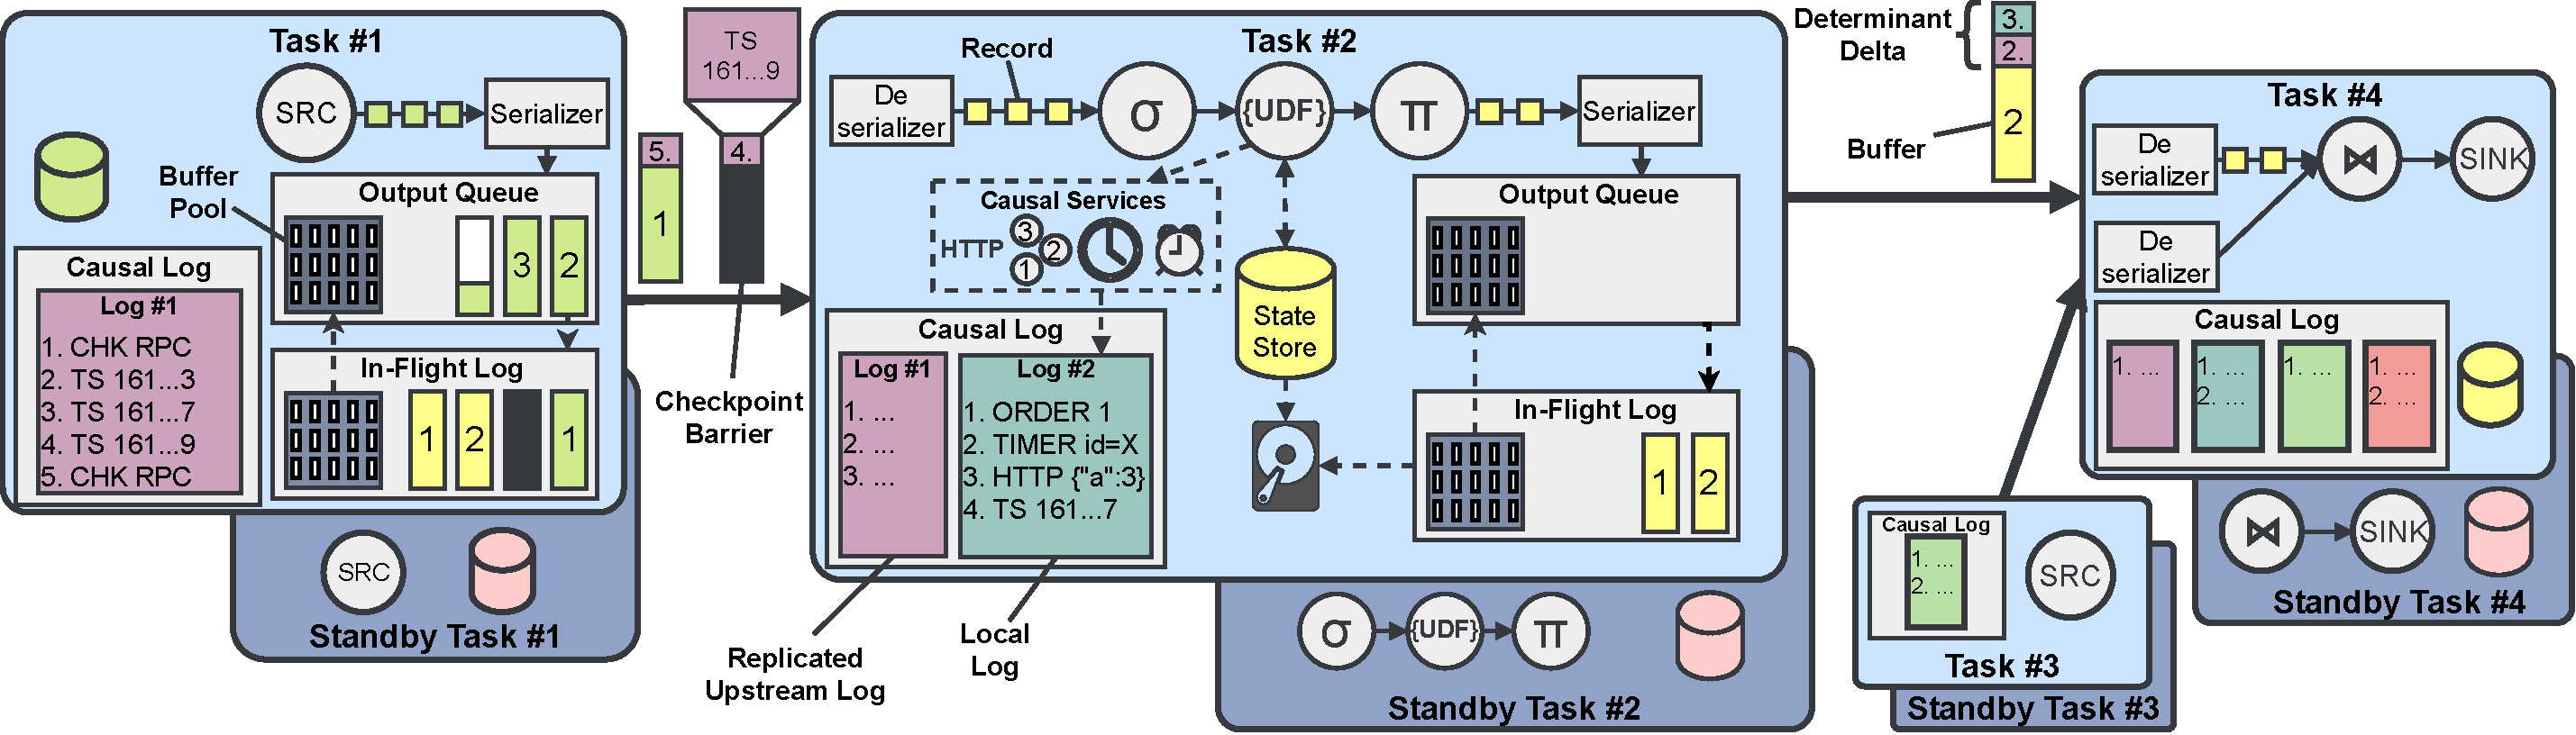
\includegraphics[width=.98\textwidth]{Figures/normal-op.pdf}
  \vspace{-2mm}
  \caption{Approach overview.} %\color{red}{FIXME!}
  \label{fig:operation}
  \vspace{-2mm}
\end{figure*}


State of the art stream processing systems can provide exactly-once processing and high-availability under failures, but by design they have grown to support specific types of workloads summarized as analytics functions, for instance aggregates and joins.
These computations, which are associated with streaming systems since their early times, are mostly deterministic and operate solely within system boundaries.
In contrast, emerging classes of applications, such as general event-driven Cloud applications~\cite{Katsifodimos2019Operational, Carbone2020beyond}, and Stateful Functions~\cite{akhter2019stateful, cloudburst} involve custom nondeterministic business logic and frequent interactions with external systems and databases.
Because of their event-based nature and performance requirements, such applications are increasingly executed as dataflows on stream processors.
To support these applications effectively, dataflow systems need to embrace nondeterminism in their fault tolerance and high availability approaches.

%State of the art fault tolerance approaches assume determinism: once a topology fails and is being recovered, it should generate the exact same events as if it never failed. However, this is a very strong assumption in practice as more and more dataflow systems are being used for executing general event-based Cloud applications \cite{Carbone2020beyond} and those include running complex, non-deterministic decisions and calling external systems and databases. 
% For instance consider the banking industry: a streaming system that rejects a banking transaction, after consulting external services needs to be auditable. Audits actually require means of tracking all sources of nondeterminism in order to be able to reason about certain actions when needed.
% For instance, consider auditing systems to ensure compliance to requirements e.g., in the banking industry. Auditing requires the means of tracking all sources of nondeterminism in order to be able to reason about certain actions when needed. Consider a streaming system that rejects a transaction, after consulting external services and the person
%Processing streams in a distributed manner is another source of nondeterminism: ingestion- and processing-time windows are nondeterministic since their results depend on local system timestamps. 
%Moreover, even event-time windows that use low-watermarks and timeouts  are not deterministic: those also use local system time to determine lateness \cite{akidau2015dataflow,CarboneKE15}. All these sources of nondeterminism have a very big effect on the applicability of streaming systems, and raise the bar for the technology to be used more in practice. 


Existing fault tolerance and high-availability approaches~\cite{Hwang2005HAA,BalazinskaBM05, Shah2004highly, delmonte2020rhino, ArmbrustDT18} fail to address the exactly-once processing guarantees in the presence of nondeterministic computations, mainly because they make very strong assumptions that are not satisfied in modern stream processing workloads. Streamscope~\cite{LinHZ16} and Timestream~\cite{QianHS13} assume deterministic computations, which restricts their applicability in practical scenarios while SEEP~\cite{migliavacca2010seep} and Rhino~\cite{delmonte2020rhino} additionally assume records to be timestamped with a monotonically increasing logical timestamp, failing to support out-of-order processing~\cite{li2008out}, which is supported by the majority of modern streaming systems today.
Finally, Millwheel~\cite{akidau2013millwheel} is the only system that does not make these assumptions, but it requires a specialized transactional backend, such as Spanner~\cite{spanner}, which requires atomic clocks not found in commodity clusters. 

In this paper we propose Clonos, a fault tolerance and high-availability method built on top of Apache Flink with the goal of supporting all existing workloads that Flink supports today, i.e., Clonos, as opposed to related work, supports nondeterministic computations. Although Clonos was built and tested on Apache Flink~\cite{CarboneKE15}, it can be used in any stream processor that simply supports FIFO per-partition channels and coordinated checkpoints~\cite{chandy1985distributed}.
In this paper we make two important contributions. First, we describe a protocol and the associated system components to perform local recovery without the need to restart a complete streaming topology, aiming at high availability and low latency with exactly-once processing guarantees. No existing work has addressed this problem on a feature-rich production-grade system. Second, we deal with the inherent nondeterminism of practical stream processing workloads in a manner transparent to application programmers.

To build Clonos, we implemented in-flight record logs and lineage-based replay for local recovery, standby tasks and live state transfer for high availability, and causal logging~\cite{elnozahy1992manetho} for exactly-once consistent execution of nondeterministic computations and system functions. We present the recovery protocol, the high-availability mechanisms, the means to track nondeterminism, and a set of noteworthy system design and implementation decisions that render Clonos a practical replacement for Flink's fault tolerance mechanism. In short, with this paper we contribute:
\begin{itemize}
  \item a novel fault tolerance approach that combines checkpointing, standby operators, and causal logging to:
  \begin{itemize}
    \item provide exactly-once consistent local recovery and high availability on a production-grade system, and
    \item support nondeterministic computations and system functions
  \end{itemize}
%  \item A drop-in replacement for a real world system without making simplifying assumptions
    \item an analysis of nondeterminism in stream processing and how Clonos guarantees exactly-once processing
  \item thorough empirical experiments carried out in a realistic deployment
\end{itemize}

The rest of the paper is organized as follows.
Section~\ref{sec:overview} offers an  overview of our fault tolerance approach.
Section~\ref{sec:background} outlines the stream processing model used in the paper and includes preliminaries regarding rollback recovery, causal logging, and Apache Flink's execution model.
Section~\ref{sec:nondeterminism} analyzes nondeterminism in stream processing and how it is addressed with Clonos, while \autoref{sec:correctness} shows how Clonos guarantees exactly-once processing.
Section~\ref{sec:design} reports important design decisions necessary to make Clonos practically appliable.
Finally, Section~\ref{sec:experiments} presents a broad set of experiments and Section~\ref{sec:related-work} 
presents related work. We conclude in Section~\ref{sec:conclusions}.


\begin{figure*}[!t]
\centering
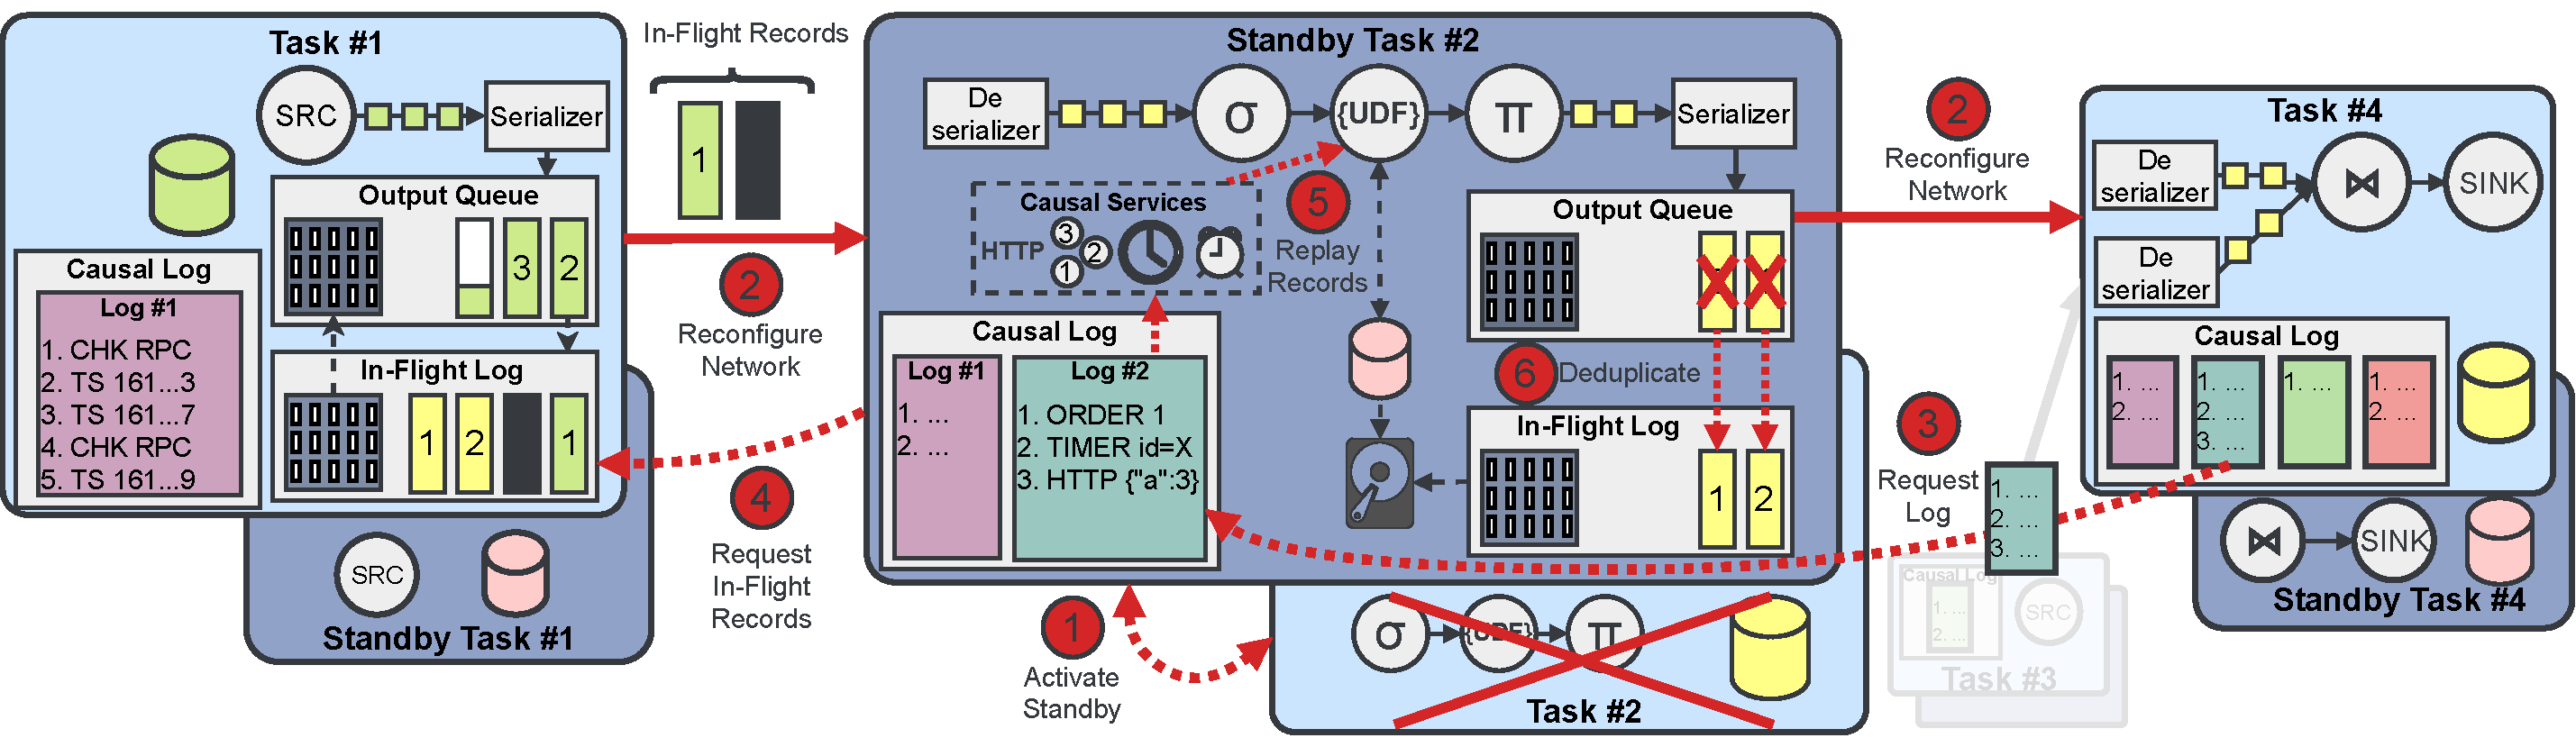
\includegraphics[width=.95\textwidth]{Figures/recovery.pdf}
\vspace{-2mm}
\caption{Steps of the fault recovery protocol.}
\label{fig:recovery-protocol}
\end{figure*}


\section{Approach Overview}
\label{sec:overview}
Clonos' main goal is to localize the impact of a failure to the minimum: only failed tasks need to recover from failure, and their upstream and downstream tasks take minimal action towards helping the failed tasks to recover.  %Treating failures locally is a fundamental aspect of Clonos and the default mode of its operation that we call local recovery mode.
Recovering locally with exactly-once processing guarantees is challenging: in order to recreate the local state of the failed task, we need to use the most recent checkpoint of that task, and replay all the input records whose effects (on the state) have not been checkpointed. 
Another difficult problem is record deduplication: because some of the records have already been produced by a failed task, the recovery protocol needs to ensure that those messages are only processed once.
The problem becomes even harder for nondeterministic computations that may produce different output (and operator state) for the same input across executions. Achieving all this in a highly-available manner where recovery has to be blazingly fast and the impact to the system's performance minor, is very challenging.
Besides local recovery, Clonos features a high availability mode where it uses standby tasks with preloaded state to speed up recovery and further lower the impact of a failure.
Below we give an overview of our recovery protocol.

\subsection{Normal Operation}
\label{sub:protocol-actions-op}

Figure~\ref{fig:operation} depicts a simple job with four tasks and their corresponding standbys. Each task executes a set of operators.

\para{In-Flight Records}
These are records that have been produced by an operator since the last successful checkpoint;
i.e. their effects have not yet been recorded to the downstream operators' state.
Tasks that send their output to downstream tasks (\#1, \#2, and \#3) maintain a log of the in-flight records in memory until the next checkpoint is
complete.
This practice is the foundation of the upstream backup strategy~\cite{Hwang2005HAA}.

Figure \ref{fig:operation} captures a snapshot of the execution when the job is processing records of the yellow epoch. 
When a record reaches Task \#2, it is processed and the output record (assuming for simplicity a function that produces a new record for each input record) is put in the output queue. Once the output record is transmitted over the network, it is added in the in-flight log.
The in-flight log is segmented into epochs, such that whenever a checkpoint completes, all records in epochs prior to the checkpoint can be removed. % Should not talk about recycling (implementation detail)

\para{Log of Nondeterministic Events}
Tasks maintain a log~\cite{elnozahy1992manetho} of determinants for recording information about nondeterministic events and operations.
In addition, each task shares its log incrementally with downstream tasks as we describe in Section~\ref{sub:causal}.
We present the different types of nondeterministic events and operations in Section~\ref{sec:nondeterminism}.

\para{Standby Tasks \& State Snapshots}
In high availability mode Clonos deploys standby tasks that mirror operator state, but remain idle in that they do not take part in data processing.
Each standby task receives state snapshots of its corresponding running task after each checkpoint.

\subsection{Recovery protocol}
\label{sub:protocol-actions-recovery}

Let's assume that right after the execution snapshot depicted in Figure~\ref{fig:operation} a failure kills task \#2.
Figure~\ref{fig:recovery-protocol} highlights the steps of our recovery protocol.% This protocol is implemented by a per-task component, the \textit{Local Recovery Manager}, which is not represented.

%\para{1. Failure Detection} 
%The upstream and downstream operators of the failed operator detect the failure through the persistent network connection and inform the job manager (not shown in the figure).

\para{1. Activate New/Standby Task}
The job manager initiates the fault recovery procedure, which starts a replacement task. In high availability mode, the topology maintains shadow/standby tasks that already contain the latest checkpointed state and remain idle until they are instructed to run by the job manager.

\para{2. Reconfigure Network Connections}
The standby task dynamically connects with the upstream and downstream task(s) of its predecessor in the topology.

\para{3. Retrieve Determinant Log}
The recovering task retrieves its predecessor's determinant log from its downstream task(s).

\para{4. Request In-Flight Records}
In parallel to step 3, the standby task sends an in-flight log request to its upstream task(s) which specifies the epochs to replay. 


\para{5. Replay In-Flight Records}
Each upstream task replays its in-flight records for the requested epoch and channel. In this case task \#1 will replay the records of the yellow and green epoch in order.
The recovering task (task \#2) begins processing these records. Whenever it reaches a nondeterministic operation, the task instead reads from the determinant log the expected result of the operation.
%Other actions (such as timers) occur asynchronously to the main processing loop and must be treated as explained in Section \ref{sec:determinants}.

\para{6. Deduplicate Output}
In parallel to step 5, the recovering task uses its determinant log to ignore output that its predecessor produced before failing.
These output records are instead used to rebuild the in-flight log state.

\noindent Clonos' recovery protocol differs in a number of ways
from upstream backup~\cite{Hwang2005HAA} where upstream tasks replay the output records to recovering downstream tasks.
Specifically, our protocol:
\vspace{-2mm}
\begin{itemize}
\item uses checkpoints to reduce the duration of replay, 
\item uses determinants to deduplicate records at the sender following a failure, and to capture many sources of non-determinism that we describe in the paper, and
\item is optimized for the architecture and capabilities of
today's distributed streaming systems, which feature shuffles, asynchronous data transfer,
checkpoints, processing-time semantics, out-of-order processing, and communication with external services.
\end{itemize}

\subsection{Applicability \& System Requirements}
Clonos makes two assumptions. The first is the existence of reliable FIFO channels between a pair of tasks, i.e., for each channel, the downstream task receives all records in the same order that the upstream task has produced them. 
The second assumption is a checkpoint mechanism that creates snapshots of the system's global state in regular intervals. Although our concrete implementation of Clonos is in Apache Flink v1.7, both assumptions are satisfied by mainstream streaming systems. For instance, Apache Samza~\cite{NoghabiPP17}, \textsc{ibm} Streams~\cite{SilvaZD16}, and the latest version of Spark~\cite{ArmbrustDT18} also provide such FIFO channels, while Streams, Jet and Trill support checkpoints.
Clonos' approach can also be easily adapted to systems using uncoordinated checkpoints, through the use of backwards flowing checkpoint complete notifications.


% We chose Flink because it is a scalable open-source distributed streaming system with a continuous processing model and consistent fault tolerance with respect to the system's state.
Clonos' implementation requires extending multiple system components such as the job manager, scheduler, checkpoint \& fault tolerance mechanisms, the network stack, and the base stream operators.
% Of all extensions to Flink, we highlight the implementation of Clonos' failure detection, causal logging, and in-flight logging mechanisms.
Clonos' implementation is available online.\footnote{\url{https://github.com/delftdata/Clonos}}


\section{Preliminaries}
\label{sec:background}

This section provides the necessary background on the concepts used throughput the paper. We focus on current recovery mechanisms for stream processing and how these relate to rollback recovery schemes and causal logging.


\subsection{Streaming Model}
Stream processing systems~\cite{akidau2013millwheel, CarboneKE15, SilvaZD16, NoghabiPP17} process unbounded collections of \textit{records} continuously by ingesting them into a dataflow graph where \textit{edges} denote record streams and \textit{vertices} denote operators.
Each \textit{operator}, receives records from an upstream operator, applies a computation on those records, and produces  output records that it sends to the next operator(s) \textit{downstream}. Each operator that produces output retains \textit{output buffers} for sending output records downstream efficiently in batches.


\subsection{Checkpoint-based Rollback Recovery}

The main fault tolerance mechanism in modern scale-out streaming systems such as Apache Flink, IBM Streams, Trill, and Jet, is converging towards periodic Chandy Lamport-style~\cite{chandy1985distributed} checkpoints of the system's global state~\cite{CarboneKE15, CarboneEF17, ChandramouliGB15, SilvaZD16}.
To recover from a failure, systems roll back the state of all operators to the latest checkpoint and resume data processing from a specific input offset, possibly replaying part of the computation that was lost during failure.
This stop and restart strategy can achieve \textit{exactly-once} processing guarantees \cite{CarboneEF17}: the effects of all input records will affect the system's operator state exactly-once. However, as the execution graph grows, so does the downtime and latency incurred by the restart. In the event of a single failure the complete execution graph needs to be torn down and restarted from the latest global checkpoint. 
%However, this approach suffers from high downtimes and latency.

This can be fixed with local rollback recovery schemes that, in-addition to the checkpoint also store in-flight records: a copy of all records they have produced since their last checkpoint. If a task fails, the system can roll back to its last checkpoint and replay its incoming records from the upstream tasks. Local recovery approaches that use in-flight logs \cite{migliavacca2010seep, FernandezMK13} can recover faster, but require two restrictive assumptions:
$i)$ that operators are deterministic (\autoref{sec:nondeterminism}), i.e., reprocessing the same record a second time will yield the same output, and
$ii)$ that each record can be identified uniquely via a logical timestamp. During replay, tasks downstream from the failure can apply dedupication using these timestamps. Clonos lifts those long-standing restrictions using causal logging.

\subsection{Log-based Rollback Recovery}
\label{sec:logging}

Log-based rollback recovery has been extensively studied in the context of distributed systems. A stream processing system can be seen as a message-passing system executing processes that send and receive messages. In the sequel, we will refer to messages as \textit{records}. 
Log-based approaches rely on the \emph{piecewise deterministic assumption}~\cite{elnozahy2002survey}, which states that all nondeterministic events can be identified, and the system can log their determinants.
To reproduce a nondeterministic event\footnote{Not to be confused with \emph{stream events} which are used interchangeably with records in database research nomenclature.} $e$ (e.g., a timer, a random number, the result of a call to an external service/system), one must store the event and its \textit{determinant}, denoted by \#$e$. 

However, having the determinants alone is not enough to replay the nondeterministic events. To replay record reception events, it is required that the record contents be replayed as well. This can be done in one of two ways: $i)$~either the receiver can log the record contents together with the determinants or $ii)$~the sender can keep a log of the sent messages that are not yet stable in a so-called \textit{in-flight record log}. The second case is more common, because the first requires logging a large number of messages in stable storage.
Instead, the in-flight record log can be kept in volatile memory,
because after a failure it can be deterministically rebuilt using the
input streams and determinants.

\subsection{Causal Logging}
\label{sec:causal_logging}

Causal logging~\cite{alvisi1998message, elnozahy1994manetho} is a log-based rollback recovery approach particularly well-suited to stream processing. 
Unlike \textit{pessimistic logging}, causal logging maintains the determinant log in-memory and unlike
\textit{optimistic logging} it ensures the \textit{always-no-orphans property}~\cite{alvisi1996understanding} (Equation \ref{eq:always-no-orphans}), allowing for localized recovery.
An orphan process is defined as a process whose state depends on a nondeterministic event $e$ that cannot be reproduced during recovery~\cite{elnozahy2002survey}. 
If a nondeterministic event cannot be reproduced, then the state of orphaned processes must be rolled back to before that event, in order to ensure consistency.
%The always-no-orphans property (Equation \ref{eq:always-no-orphans}) is used to reason about the effects of a nondeterministic event $e$:
\begin{equation}\label{eq:always-no-orphans}
  \forall e: \square(\neg \Stable(e) \implies \Depend(e) \subseteq \Log(e))
\end{equation}

\noindent where $\Depend(e)$ is the set of processes whose state was affected by $e$ according to the \textit{happens-before} relationship. $\Log(e)$ is the set of processes that have logged $e$'s determinant in volatile memory and $\Stable(e)$ is a predicate which becomes true when $e$'s effects are stored in stable storage (i.e. checkpointed). Finally, the operator $\square$ is the temporal always operator. %It is thus apparent that this is a safety property of the system.

Causal logging ensures that either $i)$ all processes that depend on $e$ have logged its determinant or $ii)$ $e$ is stable. If a set of processes $\mathcal{F}$ fails, then for all non-stable events $e$ either $\Depend(e) \subseteq \Log(e) \subseteq \mathcal{F}$, in which case there is no orphan, or $\Depend(e) \subseteq \Log(e) \nsubseteq \mathcal{F}$ in which case at least one surviving process has the determinant of e, and can share it with the recovering processes. %In order for a process to message the outside world, it must ensure that the determinants it depends on are stable, however this can be done with no coordination.

Causal logging can be optimized by ensuring that no unnecessary determinants are sent to processes that do not depend on them by strengthening the always-no-orphans property as follows.
\begin{equation}\label{eq:causal}
\begin{multlined}
  \forall e: \square ( \neg \Stable(e) \implies \\
  ((\Depend(e) \subseteq \Log(e) \wedge \diamond (\Depend(e) = \Log(e)))))
\end{multlined}
\end{equation}

This property conveys that, while $e$ is not stable, all processes dependent on $e$ must have logged it and  -- eventually $\diamond$ -- the ones that have logged it will be no more than those who depend on it. 
However, processes only depend on events of other processes if they receive  messages from them, because those events happened before the delivery of the message. Thus, there is no need to send extra messages containing determinants, since the determinants a process needs can be \textit{piggybacked} on the message that makes it causally dependent on those determinants.

Finally, in causal logging if the number of possible concurrent failures is bound to be not greater than a value $f$, it is possible to implement stable storage while avoiding disk access by logging to $f + 1$ processes~\cite{alvisi1993nonblocking}.
%This observation forms the basis for \textsc{fbl}\cite{alvisi1993nonblocking} protocols. The adapted correctness property for \textsc{fbl} is shown in \ref{eq:causalbounded}.
In this case, one process may avoid sending its determinants to processes that have not logged them, if enough processes have already logged them for them to be considered stable. %Causal logging can reduce overhead by avoiding stable storage entirely, even during output commit. %Implementations for $f = 1$ have been shown to have very small overhead\cite{alvisi1996understanding}. Another special case is when $f = N$, which is the protocol that Manetho\cite{elnozahy1992manetho, elnozahy1994manetho} implements.
\begin{equation}\label{eq:causalbounded}
\begin{multlined}
\small
  \forall e: \square ( (|\Log(e)| \leq f)  \implies \\
   ~~~~~~~~((\Depend(e) \subseteq \Log(e) \wedge \diamond (\Depend(e) = \Log(e)))))
\end{multlined}
\end{equation}



\section{Dealing with Nondeterminism}
\label{sec:nondeterminism}

Nondeterminism causes a lot of issues with the recovery of streaming topologies. The main issue arises when, upon failure and recovery, one needs to deduplicate records which have been generated twice, during replay. If the recovering operator (the one producing the duplicates) is deterministic, downstream operators can simply eliminate the duplicate records, because they know they have received them before. However, if the recovering operator is nondeterministic, it means that upon recovery, it may generate different records and/or in a different order. In that case, the downstream operators cannot correctly eliminate duplicates as they cannot distinguish them from non-duplicates. This is a very simplistic example of the relationship of local recovery schemes and determinism.  Clonos is the first local recovery scheme to offer exactly-once processing guarantees in in the lack of determinism by tracking all sources of nondeterminism, and by leveraging causal logging.

\para{Causal Logging for Stream Processing} Clonos leverages causal logging \cite{elnozahy1994manetho} to address the issues of nondeterminism. Unlike message-passing systems, the dataflow operators that process a streaming query are multi-threaded, including threads for data processing, timers, networking, flushing and receiving RPCs. Most of the different threads affect state and generate records at arbitrary system time that affect processing. In addition, a stream processing  system offers operations that rely on system or processing time, such as processing time windows. All of these nondeterministic computations and functions need to be controlled in order to provide replayable job executions in a streaming system.

\vspace{1mm}
In the rest of this section, we analyze the sources of nondeterminism (Section~\ref{sub:nondeterminism}% and Table~\ref{tab:causal-log-determinants}
), and elaborate how we deal with them (Section~\ref{sec:determinants}) including what we term \textit{causal services} -- a programming abstraction to support nondeterminism for system programmers but also to users authoring UDFs. In Section~\ref{sub:causal} we present the causal log and in Section~\ref{sec:correctness} we discuss how Clonos guarantees  exactly-once processing. Figure~\ref{fig:causal_log} depicts the concepts discussed this section.


\subsection{Sources of Nondeterminism}
\label{sub:nondeterminism}

We now exhaustively list the sources of nondeterminism that can be found in most modern stream processing systems. 

\para{Windowing \& Time-Sensitive Computations} Streaming computations very often manipulate the inherent time dimension of data, which is based on event-, processing-, or ingestion-time. Of those, processing-time and ingestion-time are nondeterministic because they rely on the local system time at the operator where they are being processed. More specifically, when processing ingestion-time windows, the source operator simply adds a field in the record marking when that record entered the system.  Upon a failure and replay, the ingestion time will change (the system time at the sources has changed), and windowing computations may not return the same results. The same holds for processing-time windows, which, instead of taking into account the ingestion time of records, simply trigger in periodic moments in time using \textit{timers}, based on the local clock of the windowing operator.
% Clonos addresses this issue, as we will see in the next section, by logging all local timestamps and replaying those original timestamps on replay.




\para{Event-Time Windows \& Out-Of-Order Processing} Event-time is quite different to processing-time. It is the time the records are generated in the input sources (e.g. sensors and mobile devices). In its simple form it is deterministic: no matter how many times one replays a stream, the event-time of each record does not change. However, event-time introduces another complexity: the possibility of records arriving from input sources out-of-order due to network congestion or other reasons~\cite{srivastava2004flexible}. Streaming systems like Google Dataflow, Apache Beam \& Flink accept out-of-order events up to a \emph{lateness bound} based on a low-watermark~\cite{li2008out}: a marker generated  at the input sources according to wall clock time that is then embedded in the data stream. 
%It consists of a timestamp that signifies that all records with an older timestamp should have reached their destination and allows the receiving operator to progress its event time and fire event-time windows when the lateness bound expires. 
Since low-watermarks are generated according to wall clock time, using timers, they are nondetermistic.

\para{Timers} Timers are programmatic hooks which can be set to execute at some point in the future. Both the system and users can register timers. The triggering of timers is controlled by a timer thread, and the interleaving of operations between two threads is nondeterministic.

% \begin{table}[t]
%   \small
%   \caption{Causal log determinants}
%   \label{tab:causal-log-determinants}
%   \vspace{-4mm}
%   \begin{tabular}{p{0.15\textwidth}|p{0.25\textwidth}}
%   \toprule
%       \textbf{Determinant type} & \multicolumn{1}{c}{\textbf{Usage (internal, users)}} \\
%       \midrule
%       Timer/timestamp & users \& internal (low watermarks, lateness measures, checkpoint times, etc.)\\\hline
%       Random number & user-defined functions\\\hline
%       Input channel order & internal\\\hline
%       Checkpoint injection & internal\\\hline
%       Buffer built size & internal\\
%       \toprule
%   \end{tabular}
%   \vspace{-5mm}
% \end{table}



\para{User-Defined Functions \& External Calls} User-defined functions are not sandboxed: they are allowed to call external services, reach external key-value stores, and also make other asynchronous calls. Every interaction with the outside world is not expected to be deterministic. Consider, for example, a call to an external database that queries the current stock price; this can change at any point in time. As a result, calling external services cannot be considered deterministic and, during recovery, computations can change. 

\para{Random Numbers} Users may want to use random numbers in operators. Pseudo-random number generators are typically initialized using the current time producing nondeterministic results.

\para{Keyed Streams \& Record Arrival Order} To parallelize and group streams, it is common to partition them using a partitioning key. We refer to such a stream as a keyed stream. 
Downstream operators (e.g. a \texttt{reduce} operator) receive inputs from multiple upstream operators, on a per-key basis. The issue here is that, depending on the network speed, the connection between various operators, etc., the order in which records arrive is not always the same upon recovery. A lot of times, operators are order-sensitive; in that case, the operator will also generate records in a different order than the one before the failure happened. In other words, operators that process multiple inputs are not deterministic. To make it deterministic, we need to fix the order in which records are replayed on recovery (see Section~\ref{sec:determinants}).


\para{Checkpoints \& Received RPCs} Checkpoint-based fault tolerance protocols inject checkpoint barriers into the dataflow graph that instruct operators to checkpoint their state as they pass through them.
Those barriers are injected in the dataflow graph through an RPC according to the system time of the job manager (e.g., every 10 seconds). Any RPC received by a task which affects its state is nondeterministic.

\para{Output Buffers} Records are grouped into buffers before they are sent downstream. Buffers are sent either when they are full or when the downstream task demands a buffer.\footnote{To handle backpressure, streaming engines allow  downstream operators to either pause transmission or force the transmission of a buffer as soon as it contains a record.} In the latter case, the buffer might not be complete. Thus, the decision of whether the buffer will be split or not is very time-dependent and also depends on the request coming from downstream. This introduces nondeterminism in the size of buffers sent downstream that needs to be taken care of, such that the buffers can be retransmitted in the very same way during recovery.





\subsection{Abstracting Nondeterminism with Services}
\label{sec:determinants}

To hide the complexity of causal logging and recovery from users that code user-defined functions (UDFs), operators have access to ``causal services'' that abstract the complexity away. For instance, assume that in \autoref{fig:causal_log} a user-defined function calls the \texttt{Timestamp} service, which returns timestamps. 
Under normal operation, the service generates a nondeterministic timestamp and appends it in the causal log.
During recovery, when the user-defined function requests a timestamp from the \texttt{Timestamp} service (shown in \autoref{call-causal-service}), the service will instead return a timestamp read from the causal log. Users can register their own nondeterministic computations in Clonos by providing an anonymous function as in \autoref{register-causal-service}. Determinants and causal logging, as well as recovery in all cases are done transparently. Behind the scenes, Clonos applies the anonymous function as \autoref{clonos-causal-service} shows. We describe the built-in causal services below.

\para{Record Processing Order} The \texttt{Order} service is an internal service (not exposed to users), which logs the order in which input records are processed. 
For performance, this is done at the level of buffers, and each buffer is fully processed before the next is deserialized.
%Two sources of nondeterminism are computations on keyed streams and the organization of records into buffers across multiple downstream channels.
%As buffers arrive to a downstream operator instance from many input channels,
%we need to store their delivery order to enforce and reproduce it after a potential failure.

\begin{figure}[t]
  \centering
  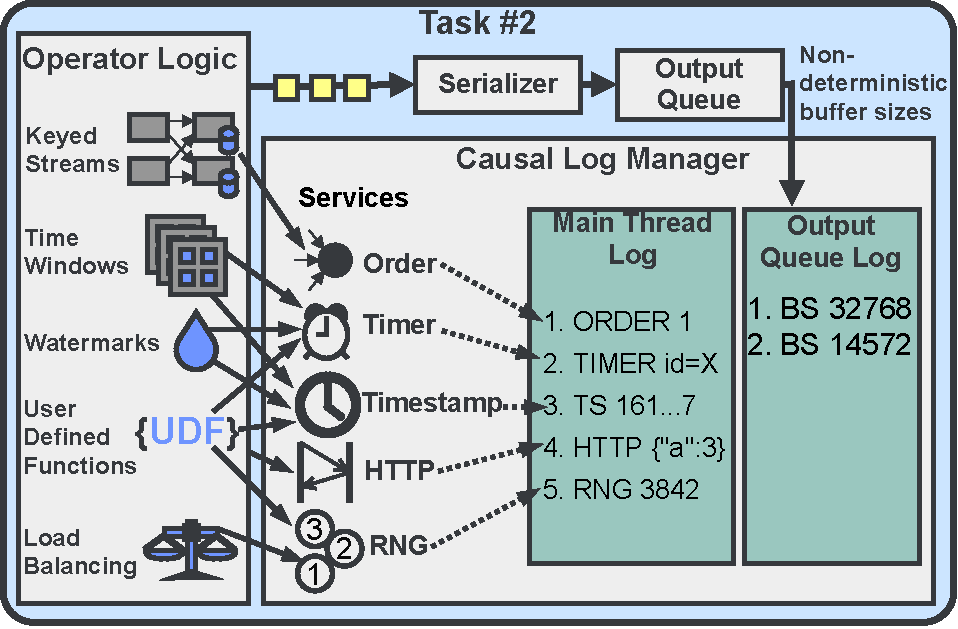
\includegraphics[width=0.8\columnwidth]{Figures/services.pdf}
\vspace{-2mm}
  \caption{Services offered by the causal log's services API.}
\label{fig:causal_log}
\vspace{-4mm}
\end{figure}





\para{Timers \& Received RPCs} Timers fire asynchronously to the main thread, thus their recovery is more complex. We first introduce unique IDs to every timer callback function. Then, we modify timer internals to register a ``TimerFired'' determinant in the causal log, containing its ID and stream offset at which it fired.
During recovery, if a ``TimerFired'' determinant is encountered, we wait for the same stream offset to be reached. We then use the timer ID to obtain and execute the corresponding callback. RPCs received by an operator are treated similarly.
% It feels like a lot of this is repeating what was said in the previous section.
%Timers are important in stream processing, as they are required for processing-, ingestion-, and event-time windows as well as progress tracking and out-of-order processing. Users may also register their own timers.
%Timers come in two variants: system timers and internal timers. System timers are used by the system for its own processing and include periodic processing-time timers for emitting watermarks, detecting stream idleness and emitting latency markers.
%Internal timers are used by streaming operators. Processing-time windows use processing-time timers to trigger window closing and result emission. Event-time windows use event-time timers to do the same, but this requires processing-time timers for watermark emission. Internal timers are checkpointed and restored. Thus, event-time timers are deterministic after failures as long as they receive watermarks, which rely on processing-time timers, at the same points.




\para{Wall-Clock Time} When the \texttt{Timestamp} service is used to retrieve wall-clock time under normal operation, the service retrieves a timestamp from the system and logs it prior to returning it to the user. During recovery, the same service will return the logged timestamp instead of a fresh wall-clock timestamp. Since this service may be called multiple times per millisecond, if the time granularity allows it (e.g., asking ms-granularity timestamps multiple times within the same ms), instead of generating a new timestamp on every call, this service utilizes timers to only update a stored timestamp periodically (each ms in this case). In between updates, the service simply returns its cached timestamp. This reduces the amount of determinants generated by two orders of magnitude without a large loss in time granularity.

\para{Calls to External Systems} Calls to external systems must be done through causal services (e.g. the \texttt{HTTP} service), which persistently record the response in the log. The response can then be deserialized from the log during recovery.

\para{Random Numbers} Instead of storing the numbers generated, the \texttt{RNG} service generates a new random seed on every checkpoint and stores it in the log. During recovery, the seed is read from the log and the numbers generated can then be deterministically reproduced.


%Moved this to later
%\para{Output Buffers} Like timers and Received RPCs, the nondeterminism in the size of output buffers sent to downstream tasks is asynchronous to the main thread. However, unlike them, these nondeterministic events are not serialized with the main thread though locks which protect operator state. We deal with this by introducing a causal log for each output channel, to which only the sizes of buffers are appended.
%We only need to create determinants for record buffers because buffers containing checkpoint barriers allow us to garbage collect determinants for the previous epoch of records.
%Thus, we do not need to track the position of a checkpoint barrier in a data stream.
%We use separate causal logs on each network thread/channel and on the main processing thread to handle asynchronous operations and distinguish records of different epochs.


\begin{figure}[t]
\begin{lstlisting}[
style=javalang,
caption=Using built-in services.,
label=call-causal-service
]
HTTPResponse response = ctx.getHTTPService().get("host:port/path");
long ts = ctx.getTimestampService().currentTimeMillis();
\end{lstlisting}

\begin{lstlisting}[
caption=Boilerplate to add a new causal service in a UDF.,
label=register-causal-service,
style=javalang, 
]
CausalService myService = ctx.buildService(input -> {
  // The user provides any nondeterministic logic and simply returns
  // an object that implements the Serializable interface.
});
//User can later use this logic with any input argument i
Output o = myService.apply(i);
\end{lstlisting}

\begin{lstlisting}[
style=javalang,
caption=Internal causal service logic.,
label=clonos-causal-service
]
class CausalService<I, O extends Serializable> {
	Function<I, O> f; //defined when service is built
  public apply(I input) {
    Output determinant;
    if (recoveryManager.running())	//Normal operation
			determinant = f.apply(input);
    else														// Recovery phase
      determinant = recoveryManager.replaySerializable();
    causalLog.append(determinant); 
    return determinant;
  } }
\end{lstlisting}
\vspace{-8mm}
\end{figure}

\subsection{Causal Log}
\label{sub:causal}

\begin{figure*}
% \relscale{.65}

\tikzstyle{nodestyle}=[text width=2cm, 
                       align=center, 
                       % level distance=.15cm, 
                       font=\sffamily]

\tikzstyle{edgestyle}=[->]

\tikzset{edge from parent/.append style={edgestyle}}

\newcommand{\redtext}[1]{\color{red}\relscale{.7}\textit{#1}}

\begin{tikzpicture}[every node/.style={nodestyle},scale=0.7]
    \centering
    \begin{scope}
    \relscale{.83}
    %!TEX root = ../hastreaming.tex


\tikzstyle{leafstyle3}=[text width=40mm, fill=myorange!40]
\tikzstyle{leafstyle}=[leafstyle3, fill=blue!15]

\tikzstyle{eqstyle}=[leafstyle3,fill=green!18, text width=8cm]
%
%
\node[fill=red!40] {\textbf{DSD $=$ D}}
        child {node[eqstyle] (ncvv1) {$\forall e: \square ( \neg \Stable(e) \implies ((\Depend(e) \subseteq \Log(e) )))$ ~~(Eq. \ref{eq:causal})}
	    % left child
	        child {node[leafstyle3, xshift=-16mm] {$\Log(e) \subseteq \mathcal{F}$ \\ (no surviving process with \#$e$)}
	        			child { node[leafstyle3] {$\Depend(e) \subseteq \Log(e)$ \\ (no surviving process depends on $e$)}
	        				child { node[leafstyle] {Recover without determinant}
	        				}
	        			}		
		        }
	%
	%
	        % right child
	        child {node[leafstyle3, xshift=16mm] {$\Log(e) \nsubseteq \mathcal{F}$ \\ ($\exists$ surviving process with \#$e$)}
	        	    % child { node[leafstyle3] {$\Depend(e) \nsubseteq \mathcal{F}$ \\ (surviving processes depend on $e$)}
		        		child { node[leafstyle] {Recover using determinant}
		        		}
	        		% }
	        }
};
%
%
\node[fill=red!40, xshift=90mm] {\textbf{DSD $<$ D}}
        child {node[eqstyle] (ncvv1) {$\forall e: \square ( (|\Log(e)| \leq \text{DSD})  \implies 
   ((\Depend(e) \subseteq \Log(e) )))$ ~~(Eq. \ref{eq:causalbounded})}
	        % left child
	        child {node[leafstyle3, xshift=-15mm] {$\Log(e) \nsubseteq \mathcal{F}$ \\ ($\exists$ surviving process with \#$e$)}
	        	    % child { node[leafstyle3] {$\Depend(e) \nsubseteq \mathcal{F}$ \\ (surviving processes depend on $e$)}
		        		child { node[leafstyle, text width=18mm, xshift=-10mm] {Recover using determinant}
		        		}
	        		% }
	        }
	    % right child
        child {node[leafstyle3, xshift=17mm, text width=35mm] {$\Log(e) \subseteq \mathcal{F}$ \\ (no surviving process with \#$e$)}
        	child { node[leafstyle3, text width=25mm, xshift=-22mm] {$\Depend(e) \nsubseteq \mathcal{F}$ \\(orphaned process)}
	        	% child { node[leafstyle3] {}
	        		child { node[leafstyle,text width=25mm,xshift=0mm] {Trigger global rollback}
	        		}
	        	% }
	        }
        	child { node[leafstyle3, xshift=0mm, text width=30mm] {$\Depend(e) \subseteq \mathcal{F}$ \\ (no orphaned process)}
	        		child { node[leafstyle, text width=34mm] {Recover without determinant}
	        		}
	        }	
        }
};
        % \draw[edgestyle]  (ncvv1) edge (hor1);

    \end{scope}


\end{tikzpicture}
\vspace{-4mm}
\caption{Exhaustive list of failure cases \& DSDs with the recovery scenarios that need to be followed in each case.}
\label{fig:recovery-cases}
 \vspace{-2mm}
\end{figure*}

The causal log stores the determinants for every nondeterministic event executed by a task. It is split in two parts. There is a causal log for the main thread of a task and a separate causal log for each of the output channels in that operator. 

In a typical message passing system with a single thread of execution, causal logging~\cite{elnozahy1994manetho} would require maintaining only one log generated by that single thread of execution.
However in a typical scale-out streaming system, the main processing thread is separate from the network threads for performance, and they communicate through shared data structures.
As the main thread writes to an output buffer, the output queue may decide to send the non-full (nondeterministically sized) buffer downstream.
Thus, each queue has a causal log, where the size of buffers sent is recorded (\autoref{fig:causal_log}). This log is used during recovery for deduplication.

\para{All Buffers Carry Determinants} Whenever a buffer of data is sent downstream, a causal log delta piggybacks on that buffer. The delta contains all the  entries of the output queue logs and the main thread log since the last buffer dispatch. Note that the main thread log is essentially replicated to all downstream operators, as formally required by causal logging~\cite{elnozahy1994manetho}. The idea behind this is that whenever a downstream operator receives determinants, those should be able to fully restore the upstream operator. 



\para{Replicating Determinants to Downstream Tasks} The downstream task, upon receiving the buffer and the delta of the two logs, appends those updates to the corresponding task causal log. In this way, before data is allowed to affect the state, the causal information necessary to recover it is already stored. In order to be able to afford two successive tasks failing, one might also want to replicate the determinants of each task to a deeper sharing depth. 

\para{Truncating Causal Logs} The causal log is organized in segments according to epochs and is truncated whenever a checkpoint completes; the causal log is only needed in the middle of an epoch, when a local recovery has to complete using in-flight logs and the older checkpoint as we describe in the next section.

\section{Exactly-once Recovery}
\label{sec:correctness}

In this section we show how Clonos deals with recovery and how it guarantees \textit{exactly-once processing} with local recovery, using a causal log and in-flight records. In \autoref{sec:exactly-once-output} we describe how we could extend Clonos to guarantee \textit{exactly-once output}.


\subsection{Lineage-based Replay}
\label{sub:lineage}


When a new task replaces a failed task it needs to process the records of the current checkpointing epoch.
Therefore, it requests from its upstream tasks to replay their in-flight record log.
Upon the in-flight log request, upstream tasks start to replay the buffers contained in their in-flight log, in the same order they were dispatched prior to failure. The replay protocol of Clonos is based on lineage.
If a task does not have an in-flight record log to replay for a downstream task (typically because itself just recovered from a failure), it will ask its upstream tasks to replay their in-flight record log.
This lineage-based process can reach recursively the operator graph all the way up to the input sources, which we assume to be available to provide their input on demand.



\subsection{Determinant-based Deduplication}
When recovering a task, the task replays the received in-flight records and produces output. Achieving exactly-once processing when performing local recovery requires deduplication after replay. In prior work~\cite{FernandezMK13}, such deduplication is rather simple: each operator is considered to be deterministic, and all produced records bear a logical timestamp. The downstream operator can simply discard the records bearing the already seen logical timestamps. However, receiver-based deduplication wastes bandwidth. 

Instead, deduplication in Clonos is done in two concurrent steps. First, as the main processing thread recovers, it uses its causal log to produce the exact same output records. Concurrently, the network channel threads use their causal logs, which contain only information about the size of buffers received downstream, to reconstruct the same buffers as sent before. %The work to perform serialization is not wasted, as these buffers are instead used to rebuild the in-flight log, in case any failures happen downstream.

\subsection{Correctness of Recovery Scheme}
\label{sec:determinant-recovery}


In the following, we analyze the conditions under which recovery can be performed using determinants depending on the depth to which determinants are shared. The correctness of causal logging as a rollback recovery approach has been formally proven in the past \cite{alvisi1996understanding, alvisi1998message}. Since Clonos tracks nondeterminism for multiple threads (the main processing thread and one thread per output channel), we model each thread as a process and recover them in unison. Thus, the proofs applicable to pure causal logging trivially extend to Clonos. However, ensuring exactly-once processing when locally recovering a failed operator remains open;
we show Clonos guarantees it in the following paragraphs.

We base our reasoning on exhaustively enumerating the different states that the recovery mechanism can reach, depending on the determinant replication strategy and different failure scenarios. Our aim is to show that independently of: $i)$~how the determinants are shared with downstream operators, and $ii)$~which failure scenario takes place, there is a mechanism to recover the topology with exactly-once processing guarantees.
This is done either by retrieving determinants and deduplicating using them or by falling back to restarting the complete dataflow graph as in reference~\cite{CarboneEF17}.

Assume that in a \textsc{dag} composed of $\mathcal{N}$ tasks with a maximum depth $D$ (source tasks have a depth of zero) $\mathcal{F} \subseteq \mathcal{N}$ tasks fail. Clonos can be configured to use a determinant sharing depth (DSD) as large as the graph depth or smaller than the graph depth.
The determinant sharing depth also defines the number of consecutive tasks that can fail concurrently without creating orphan tasks. 
For instance, a sharing depth of two, means that the determinants of a task $a$ are sent to the downstream task $b$ directly, and $b$ forwards the same determinants to its downstream tasks $c$ and $d$. If both $a$ and $b$ fail, we can recover them from the determinants that are stored by $c$ and $d$. In the following, we analyze the different recovery cases, as depicted in \autoref{fig:recovery-cases}.

\para{Case 1: $DSD = D$} We deal first with the case where the determinant sharing depth equals the depth of the dataflow graph, i.e., $DSD = D$. 
Note that in this configuration Clonos follows the condition stated in Equation \ref{eq:causal}. As such, determinants for a nondeterministic event $e$ whose effects have not yet been globally checkpointed, are propagated to all downstream processes. Determinants piggybacked on a buffer are logged by a task (processed by the causal log manager) before the operator state becomes dependent on them (before the operator processes the buffer's records), and as such at no moment do we break the condition that $\Depend(e) \subseteq \Log(e)$. 


\noindent Two failure cases can occur:
\begin{itemize}
\item $\Log(e) \subseteq \mathcal{F}$: Since the condition $\Depend(e) \subseteq \Log(e)$ also holds, then no surviving process depends on $e$, meaning that a different execution path may be taken without breaking consistency or the always no-orphans condition. 
\item $\Log(e) \nsubseteq \mathcal{F}$: At least one surviving process has the determinant of event $e$, in which case it guides the recovery, either by ensuring the main thread follows the correct execution path or by ensuring an output thread deduplicates a buffer and thus the records it contains. 
\end{itemize}

Translating this to stream processing: this case can only happen when for the failure of a given task, all downstream tasks also fail, as otherwise, downstream tasks will have the necessary determinants to bring the failed tasks into a consistent state with the surviving downstream tasks. The extreme case happens when $\mathcal{F} = \mathcal{N}$, in which case no task is dependent on any other and recovery is effectively equivalent to restoring a global checkpoint and beginning replay from the graph's input sources.

\para{Case 2: $DSD<D$} In the case where the determinant sharing depth is less than the depth of the dataflow graph, Clonos follows the condition of Equation \ref{eq:causalbounded} by not sharing $e$'s determinant to a depth greater than $DSD$. In this case, there is the possibility that $\Log(e) \subseteq \mathcal{F} \nsubseteq \Depend(e)$, meaning that some orphaned process remains.  When one of the orphaned processes receives a determinant log request from a recovering task for a log it does not have, it will escalate this to the JobManager, which will trigger a full rollback of the \textsc{dag}, thus achieving exactly-once processing guarantees. The alternative case is that $\Log(e) \nsubseteq \mathcal{F}$, in which case at least one surviving task has the determinants of nondeterministic event $e$, and can guide the recovery of the failed tasks which depend on it.


Summarizing, the recovery cases depicted in the leafs of the trees in \autoref{fig:recovery-cases}, show that there are cases $i)$~when the determinants are not required for recovery, $ii)$~when determinants are required and can be found in some surviving task, and, finally $iii)$~(the worst case) when the topology can recover with a global rollback recovery mechanism.


\subsection{Trading Correctness for Performance}
Clonos is flexibly configurable in terms of its fault tolerance guarantees. By combining its different building blocks, it can achieve different processing guarantees, as follows.


\para{At-most-once} By disabling both in-flight logging and causal logging/determinants, failed tasks will be recovered with gap recovery \cite{Hwang2005HAA}, leading to inconsistent state with at-most-once processing guarantees, but incurring very little overhead.
%Note that this approach is only supported conceptually, as due to the spanning serialization of records to buffers, Clonos cannot currently resume replay from any arbitrary point. 

\para{At-least-once} By setting the determinant sharing depth $DSD = 0$, only in-flight logging is enabled, and failed tasks are recovered with divergent rollback recovery, achieving at-least-once processing guarantees with very little overhead due to Clonos' no-copy in-flight log (\autoref{sec:in-flight-design}). 


\para{Exactly-once} By enabling causal logging it is possible to perform consistent recovery on failed tasks, providing exactly-once processing guarantees, again with little overhead. If the overhead of causal logging becomes a concern, Clonos can also trade-off determinant sharing depth for performance. The determinant sharing depth is set to the depth of the graph by default, but by lowering it to another number $f$, the determinant sharing overhead is reduced in exchange for supporting at most $f$ concurrent consecutive failures. In this case, if a larger than $f$ number of failures happens, Clonos can again be configured to favour either $i)$~availability with at-least-once guarantees (skips deduplication step), or $ii)$~consistency by falling back to recovery using the latest global checkpoint~\cite{Carbone2020beyond}.

\subsection{Achieving Exactly-once Output}
\label{sec:exactly-once-output}
There are two common methods for achieving exactly-once output\footnote{This is also known as the \textit{output commit problem} \cite{elnozahy2002survey}} in stream processing systems. The first solution is idempotent sinks~\cite{ArmbrustDT18,CUSTOM:web/Storm,CUSTOM:web/Trident} and the second is transactional sinks~\cite{ArmbrustDT18, CarboneEF17}.
The idempotent sinks do not work in the face of nondeterminism, while the transactional sinks introduce latency proportional to the checkpoint interval.
Clonos, can be trivially extended to achieve \textit{exactly-once output} by piggybacking serialized determinants on records sent to downstream systems (e.g. Kafka).
This downstream system has to store these determinants, and be able to return them when requested. The determinants of a previous epoch can be truncated after each checkpoint. 
In this way, Clonos can achieve very low-latency exactly-once output since the outputs can be consumed already by external systems without having to wait for a checkpoint to complete and the transactional sinks to perform a two-phase commit.








\section{System Design Decisions}
\label{sec:design}

In this section we detail the interesting and non-trivial design decisions of the various building blocks comprising Clonos.

\subsection{In-flight Record Log}
\label{sec:in-flight-design}

Clonos stores in-flight records in each task that sends its output to other tasks downstream.
Because an upstream task may send records to multiple tasks downstream, the records are logged by output channel (partition), which corresponds to a specific connection with a downstream task. 
To optimize throughput, Flink sends records downstream, serialized in network buffers. Clonos logs these buffers in the in-flight log before they are sent.

\para{Avoiding Buffer Copies} Normally, when a buffer is sent over the network, it needs to return to the buffer pool of the output channels and be recycled. However, the in-flight log also needs to store that buffer. One choice would be to copy it over, and then recycle the buffer. However, to avoid copying buffers, whenever a buffer is dispatched from the network layer downstream, the output channel simply hands over that buffer to the in-flight record log.
This, however, can cause deadlocks: the output channels could be waiting for buffers to become available in order to serialize output records, but no buffer would be available if they would all be used by the in-flight log.

\para{Large Buffer Pools \& Backpressure Delay} After going through multiple design and implementation iterations optimizing throughput and latency, we opted for the following strategy. As seen in \autoref{fig:operation}, each channel maintains two buffer pools. One buffer pool serves the output channels and the other buffer pool serves the in-flight log. When the network layer hands over a buffer to the in-flight log, in exchange, the in-flight log hands over an empty buffer to the buffer pool of the output channel. Interestingly, in our experiments we have seen that a network  connection between two operators needs around 10 buffers per channel - not more. Adding more buffers to output channels might look rational but it has an important side effect. It breaks the natural backpressure mechanism. The more buffers available for output, the slower the reaction of upstream operators to slowdowns from downstream operators, delaying the backpressure messages to propagate back to the sources. That is precisely the reason why Apache Flink, by default, uses a very small buffer pool for output. 

Clonos, however, has to address an additional issue owed to the small number of buffers available to the output queue.
While a task upstream of a failure replays buffers to the recovering task downstream, its main processing thread continues to produce records that very quickly fill the buffers available to the output queue as those buffers cannot be sent before the replay completes.
With no buffers available processing stops for \textit{all output partitions/channels} of the task. This issue conflicts the philosophy of Clonos that the system should never stop making consistent progress.
We solved it by placing the buffers at the back of the in-flight log even though they were still unsent. This is allowed because if the downstream is failed, then we are guaranteed to replay them at a later time.
%As we describe next, this action allows those buffers to be spilled to disk and then recycled.
%Essentially, to overcome this issue we spill buffers to disk (Figure \ref{fig:operation}) and read them back until Clonos catches up with the input or the next checkpoint happens.

\para{Spilling to Disk} Our in-flight log is segmented into epochs, and whenever a checkpoint completes successfully, the in-flight log is truncated up to that checkpoint, making the data buffers available in its local buffer pool. 
The in-flight record logs are kept in memory by default.
Depending on the checkpoint frequency  and input throughput pace, the in-flight log may grow beyond the size of the log's buffer pool leading to blocked processing and backpressure.
To counteract this issue, we introduced an asynchronously spilling in-flight log, that persists buffers to disk (Figure \ref{fig:operation}), recycling them whenever necessary.
The spilling in-flight log transitions seemlessly from on-disk buffers to in-memory buffers and prefetches on-disk buffers to speed up the replay process. It functions according to the following four (configurable) policies.

\begin{itemize}
    \item In-memory: keep all buffers in memory.
    \item Spill-epoch: spill each epoch as soon as the next one starts.
    \item Spill-buffer: spill each buffer as it arrives.
    \item Spill-threshold: Spill all buffers whenever the buffer pool's ratio of available buffers drops below a configurable fraction.
\end{itemize}

The in-memory and spill-epoch policies both suffer from the possibility of blocking processing when the checkpoint interval is too large.
Instead, the spill-buffer approach entails additional synchronous work that creates increased overhead and lacks batching of I/O operations.
The spill-threshold approach offers a well-rounded solution to the above issues.



\subsection{Network Channel Reconfiguration}

Clonos applies reconfiguration of network channels dynamically in order to introduce a new task in the topology.
Once the new task receives the acknowledgment from an upstream task, it requests to establish a persistent network connection with its upstream tasks.
After a new connection has been setup, the lineage-based replay protocol can begin.

We found it particularly challenging to re-engineer the network stack in order to establish connections of tasks while jobs were executing. The main issue was to align network buffers and counters that match buffer sequence ids. In addition, record deserializers per input channel often keep state from one buffer to the next as they wait to receive the remaining part of a record with the next buffer.



\subsection{Standby Tasks}

Each standby task mirrors a running task.
It contains the same processing logic and stores the same type of state as the one it mirrors.
If a running task fails, its corresponding standby task substitutes it.
In contrast to a running task, its standby task remains idle unless it is commanded to run.

The allocation strategy of standby tasks underlies an important tradeoff between resource utilization and failure safety, even performance.
By controlling the affinity and anti-affinity of standby tasks' allocation, stream processing jobs can tune the amount of compute nodes they utilize for standby tasks.
Each saving in resource utilization directly reduces Clonos' safety guarantees since co-locating two or more standby tasks on the same node makes Clonos more susceptible to a potential failure of that node.

Performance is another factor to weigh in when deciding the placement of standby tasks, i.e. their allocation strategy.
Depending on a job's processing, co-locating two specific tasks may be critical for performance.
If performance optimization is more important than failure safety, a job may choose to co-locate the corresponding standby tasks.
By default, Clonos allocates standby tasks using the same allocation strategy provided by a job for the running tasks.


\begin{figure*}[t]
    \centering
    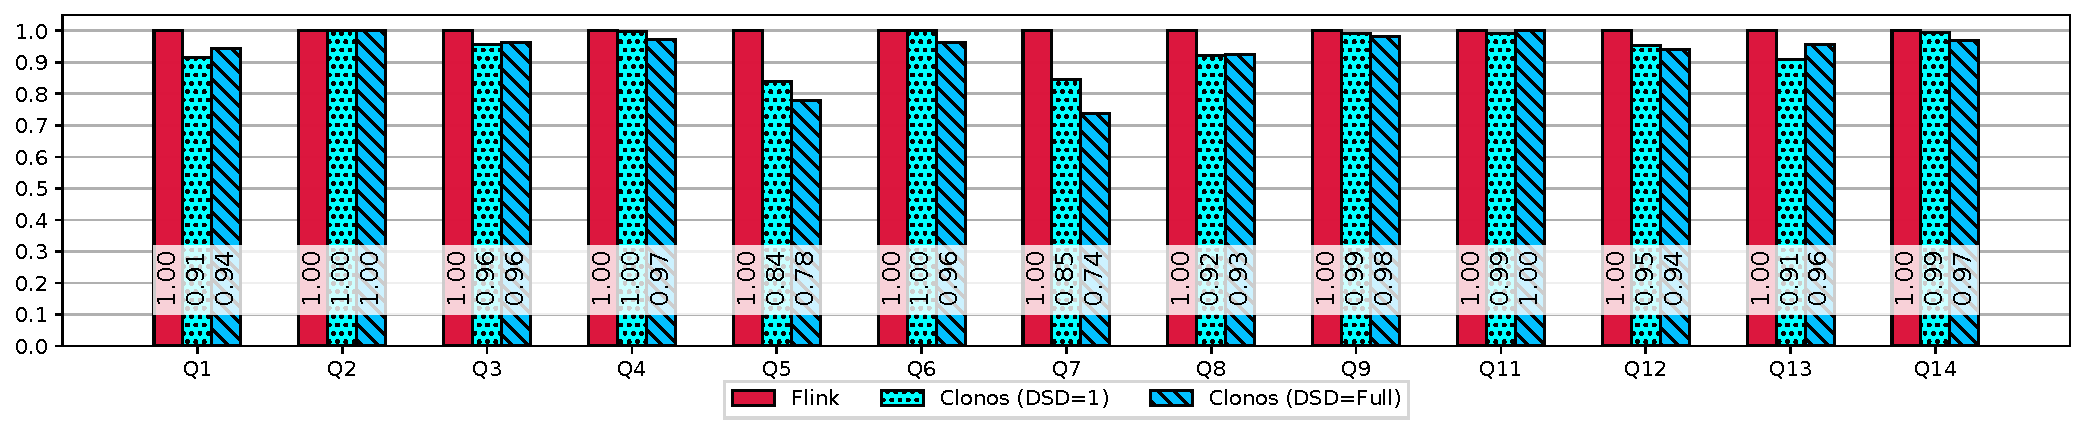
\includegraphics[width=.98\textwidth]{Figures/overhead.pdf}
    % \vspace{-2mm}
		\caption{Relative throughput of Clonos (with DSD=1, DSD=Full) compared to "vanilla" Flink's recovery mechanism, under normal operation. The experiment performed on Nexmark queries.}
\label{fig:overhead-nexmark}
\vspace{-2mm}
\end{figure*}

\subsection{State Snapshot Dispatch}

Similarly to related work~\cite{Hwang2005HAA, KwonB08}, Clonos transfers the state snapshot of each running task to its corresponding standby task once a checkpoint is complete.
Clonos' state snapshot dispatch can leverage the various approaches offered by the underlying system, such as direct transfer to the local disk of the standby task via a file url or transfer to a shared file system.
In addition, if the state backend supports incremental checkpoints then the cost of dispatching state depends on the state's delta instead of its absolute size.
By receiving state snapshots regularly, standby tasks are behind their running counterparts only by a checkpoint or less.

It is important to note that the state transfer process is bound by checkpoint frequency and checkpoint duration, which depends  on the state size.
A state snapshot should not take longer to dispatch to a standby task than the job's checkpoint frequency. 
In practice, however, this can be avoided if concurrent checkpoints are never performed.
Under these assumptions, a checkpoint is guaranteed to complete before the next one begins and state transfer is expected to complete before the next checkpoint's completion when using a distributed file system. 
Finally, if a standby task is called to run while a state snapshot is in transit Clonos will wait for the transfer to complete before starting the execution of the standby task.
% This prioritization of actions guarantees a consistent recovery.



\section{Experimental Evaluation}
\label{sec:experiments}

In this section, we first present our experimental methodology for running two categories of experiments: overhead experiments where we measure the overhead of Clonos in terms of throughput and latency under normal operation, and failure experiments where we study Clonos's fault recovery. In both cases, we compare with Flink, the engine on which our changes were introduced.% and a baseline local recovery mechanism \cite{FernandezMK14,FernandezMK13}.

% Then we formulate the questions we aim to answer with the experiments and discuss the experimental results that consist of throughput, latency and recovery time, both during failure-free operation and under failure(s).




\subsection{Setup}
\label{sub:experimental-method}

We evaluate Clonos on a Kubernetes cluster hosted on a Cloud environment. The Kubernetes cluster hosts a 3-node Kafka cluster, which serves both as the data source and data sink of the failure experiments. An HDFS deployment, with a single NameNode and three datanodes, stores the operators' checkpoints. Finally, the  Kubernetes cluster hosts a Flink cluster with 150 TaskManagers, each containing a single task slot. Each TaskManager has access to 2GB of memory, and two processing cores. 
A given configuration's throughput is measured by sampling the Kafka cluster three times per second for the number of records in the output topic. Dividing the number of new records by the elapsed time, we obtain real-time throughput.
A given configuration's latency is measured by sampling the output Kafka topics from each job and computing the output records' latency.
Finally, we configure Flink to offer the fastest possible recovery, so as to provide a fair comparison. This means lowering the failure detection parameters to values not recommended for use in production. In particular, heartbeats are sent every 4 (default: 10) seconds, timing out after 6 (default: 60) seconds.

\subsection{Workloads}
\para{Nexmark} Since Clonos can be a drop-in replacement for Flink jobs, we used the Nexmark~\cite{tucker2008nexmark} benchmark, along with the extra queries\footnote{\texttt{https://beam.apache.org/documentation/sdks/java/testing/nexmark/}} implemented by the Apache Beam project. To enable this we implemented a Clonos runner for Apache Beam. Nexmark includes queries that perform filtering, joins, aggregates, complex windowing, etc. and serves greatly as a representative workload for evaluating stream processing engines. We have excluded Q10 from the benchmark because it requires access to Google's GCP service. 

\para{Synthetic}
We also use a synthetic workload to be able to evaluate Clonos under configurable scenarios, not found in Nexmark and to avoid optimizations such as operator fusion. This way, for each operator, there is an extra layer of depth for which Clonos pays full network and serialization costs of determinants. 
For the synthetic experiments presented, we inject to Clonos multiple sequential failures, either concurrently or in intervals. In the interest of space, we only include a subset of our results.



\subsection{Overhead Under Normal Operation}
\label{sec:overhead}

In this series of experiments we observe the performance of Clonos under normal operation, i.e., without failures, and quantify runtime overheads. We execute the complete Nexmark benchmark queries setting the degree of parallelism of each operator to 25, meaning that the different jobs occupy between 25 (3 operator stages for the simplest queries such as Q1-2) and up to 150 CPU cores (6 stages for Q7). Operator fusion is turned on.



\vspace{3mm}
\begin{myframe}
\textbf{What is the overhead of Clonos in terms of latency and throughput, under normal operation (no failures)?}
\end{myframe}
\vspace{2mm}

In the interest of space, we do not plot latency measurements as we observed those to be stable and comparable to Flink's latency throughout our overhead experiments with a notable difference: the tail latency in the case of DSD=Full can be up to 20\% worse (ca. 25ms) than vanilla Flink. For DSD=1 we have noticed an overhead of less than 10\% in the worst case.

\autoref{fig:overhead-nexmark} depicts the overhead of Clonos on throughput. First, we see that for simple queries such as Q1-Q2 which are implemented with simple \texttt{map} \& \texttt{filter} operators (D=1) are not affected by the overhead that comes with Clonos, such as in-flight logging. In fact, such a small difference in throughput can easily be also attributed to the effects of the underlying infrastructure. The most complex queries are Q5 and Q7 which are implemented using an aggregation tree to handle skewed keys, and they also perform windowed aggregates. For both queries we observe that, since their depth D=6, the "Full" determinant (i.e., DSD=6) sharing has a high impact on throughput: up to 26\%. However, a more reasonable DSD=1 or 2, yields around 15-16\% overhead in throughput. We find this penalty in throughput reasonable, considering the benefits of Clonos' fast recovery times (next Section) and its ability to deal with non-deterministic operators. Finally, throughout the whole benchmark, we have observed an average penalty of 7\% for DSD=Full and 6\% for DSD=1 compared to vanilla Flink.

\subsection{Clonos Under Failure Scenarios}

\begin{comment}
\begin{table}[bt]
\small
\caption{Configurable parameters}
\label{tab:job-config}
\begin{tabular}{p{0.12\textwidth}p{0.06\textwidth}p{0.25\textwidth}}
    \textbf{Parameter} & \textbf{Default} & \textbf{Description} \\
    \toprule
    Parallelism (P) & 5 & Parallelism of each operator.\\\midrule
    Depth (D) & 5 & \# of mappers between source and sink.\\\hline
    State Size (SS) & 100MB & Amount of state held by each map operator in the graph\\\hline
    Keyed Stream (KS) & True & Shuffles between operator stages or not.\\\hline
    Operator (O) & Map & Type of operator used (\texttt{map} or \texttt{window}).\\\hline
    Time Characteristic (TC) & Processing & Processing-, Event-, Ingestion-time\\\hline
    Processing Difficulty (PD) & 620 & How complex processing each record is. Implemented through loop iterations.\\\hline
    \%  of State Updates (AS) & 0.0001\% & Probability that operator state will be modified by an event.\\\hline
    Determinant Sharing Depth (DSD) & 1 & How far Clonos replicates determinants.\\\hline
    \toprule
\end{tabular}
\vspace{-6mm}
\end{table}

\end{comment}

\begin{figure*}[!t]
	\begin{subfigure}[t]{0.25\textwidth}
		\centering
		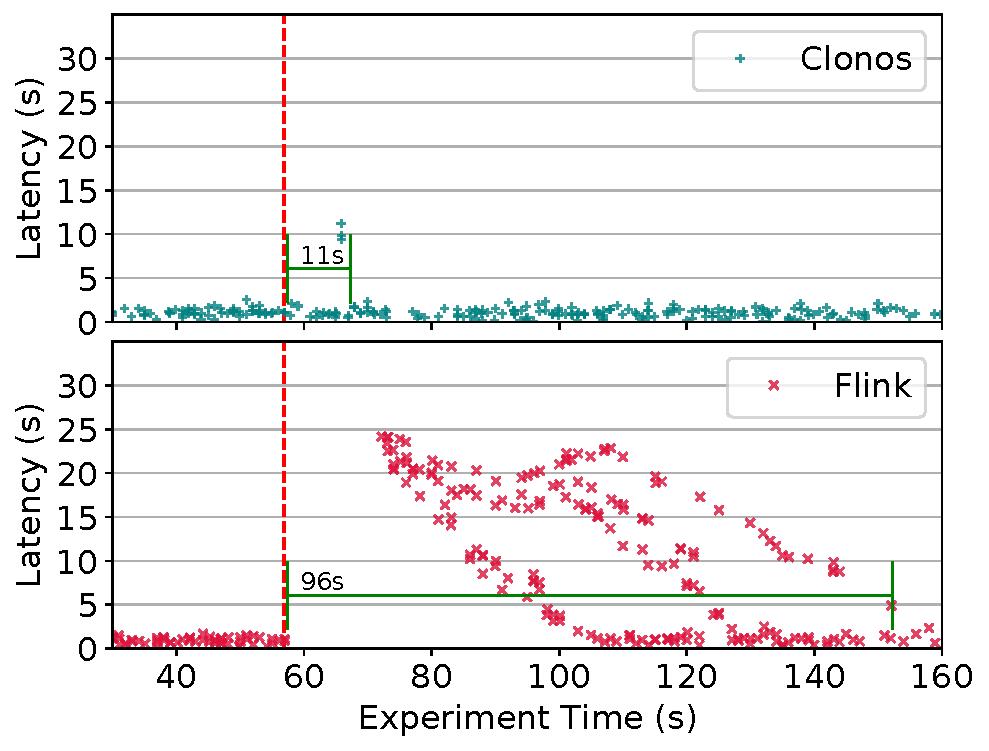
\includegraphics[width=\textwidth]{Figures/q3_failure_latency.pdf}
		\caption{Q3: latency}
		\label{fig:nexmark-q3-l}
	\end{subfigure}%
	~
	\begin{subfigure}[t]{0.25\textwidth}
		\centering
		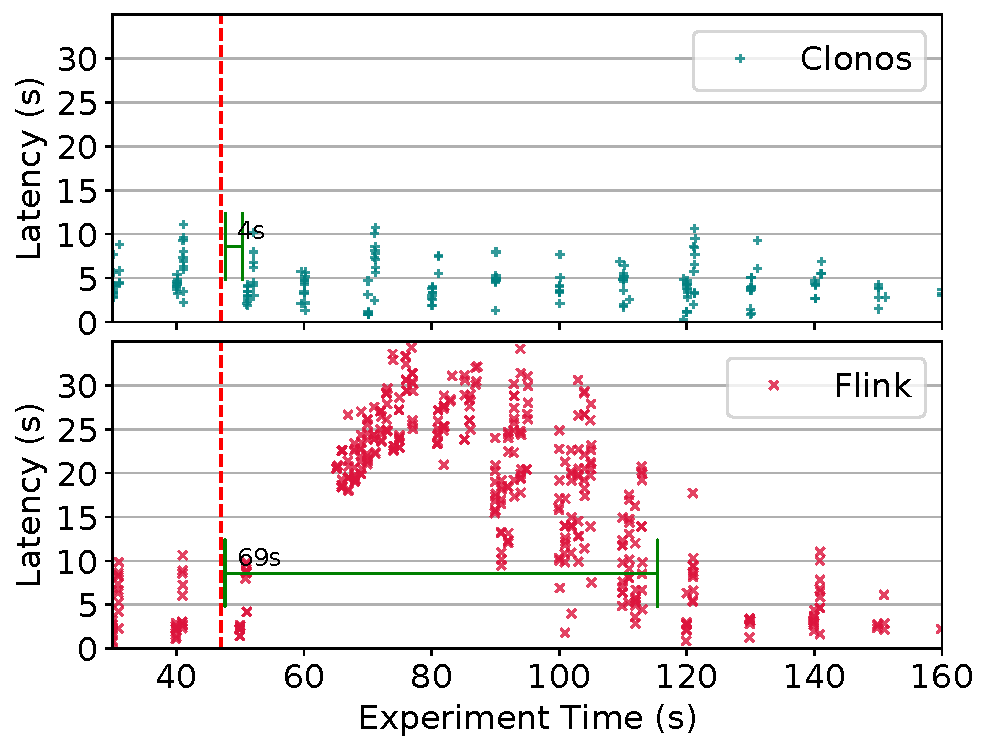
\includegraphics[width=\textwidth]{Figures/q8_failure_latency.pdf}
		\caption{Q8: latency}
		\label{fig:nexmark-q8-l}
	\end{subfigure}%
	~
	\begin{subfigure}[t]{.25\textwidth}
		\centering
		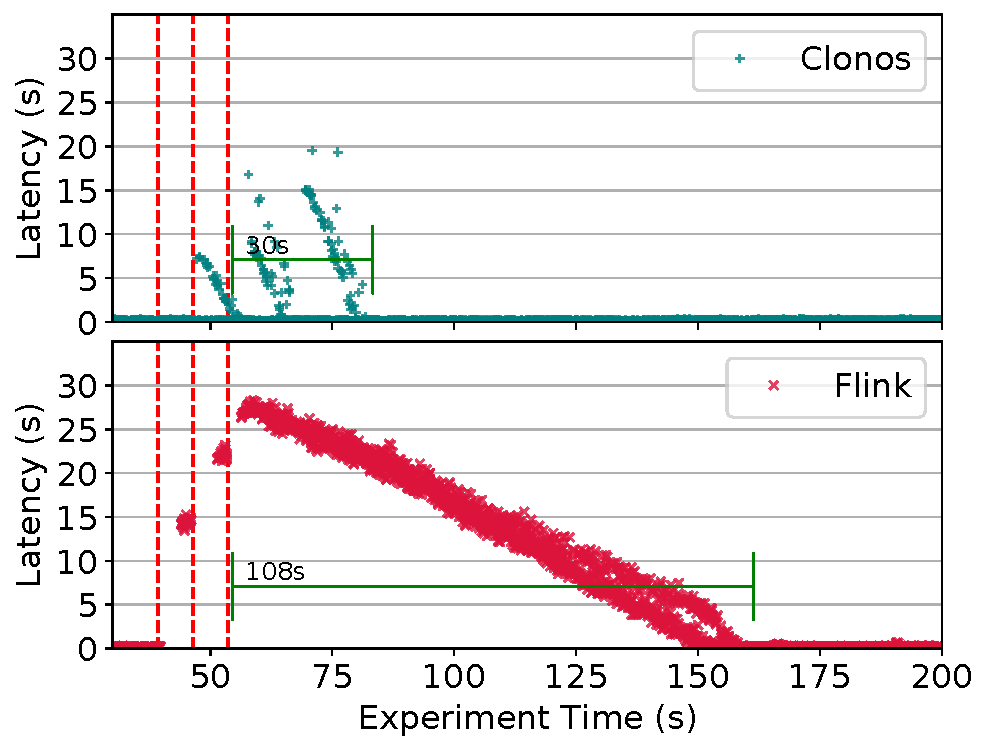
\includegraphics[width=\textwidth]{Figures/multiple_failure_latency.pdf}
		\caption{Multiple: latency}
		\label{fig:multiple-l}
	\end{subfigure}%
	~
	\begin{subfigure}[t]{.25\textwidth}
		\centering
		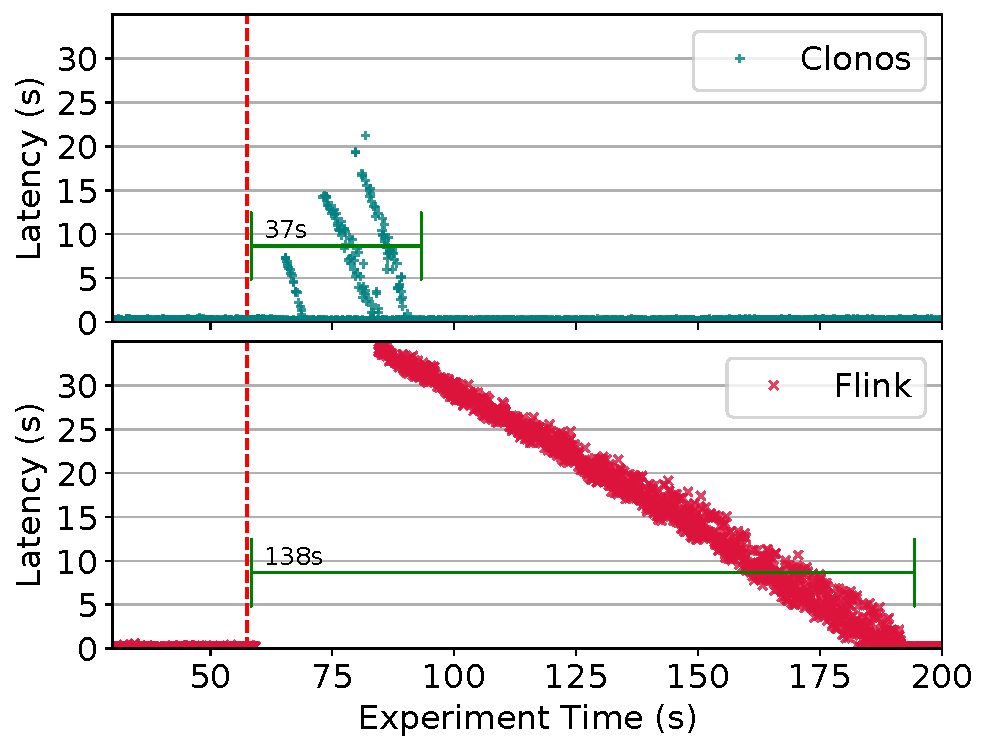
\includegraphics[width=\textwidth]{Figures/concurrent_failure_latency.pdf}
		\caption{Concurrent: latency}
		\label{fig:concurrent-l}
	\end{subfigure}%	

	% \vspace{3mm}

	\begin{subfigure}[t]{0.25\textwidth}
		\centering
		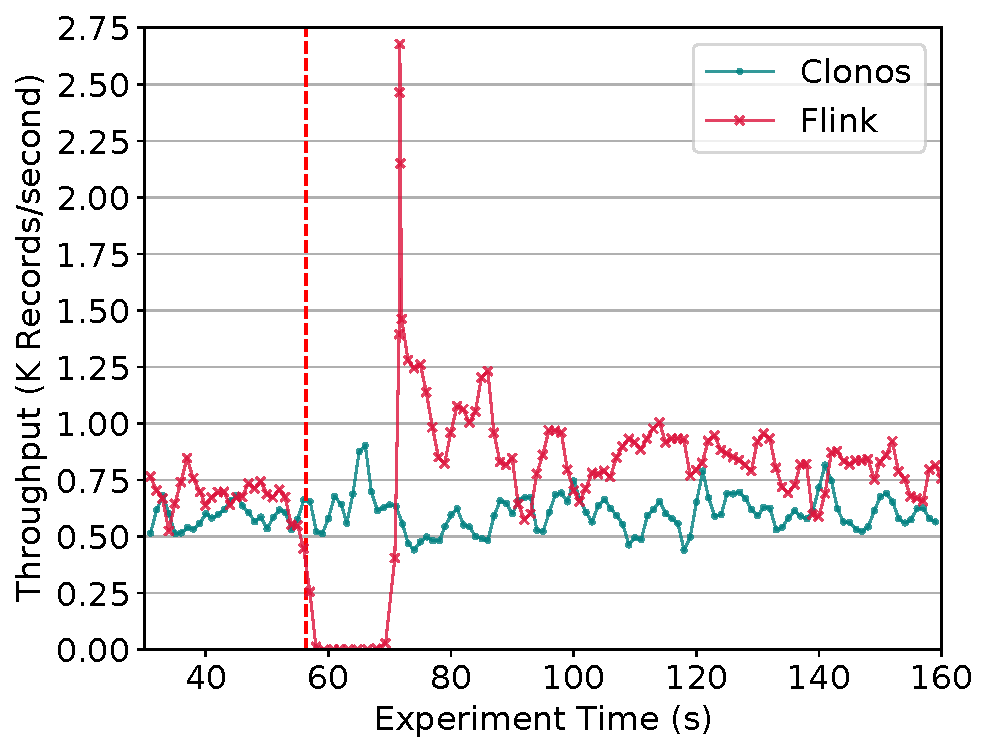
\includegraphics[width=\textwidth]{Figures/q3_failure_throughput.pdf}
% 		\vspace{-1mm}
		\caption{Q3: throughput}
		\label{fig:nexmark-q3-t}
	\end{subfigure}%
	~
	\begin{subfigure}[t]{0.25\textwidth}
		\centering
		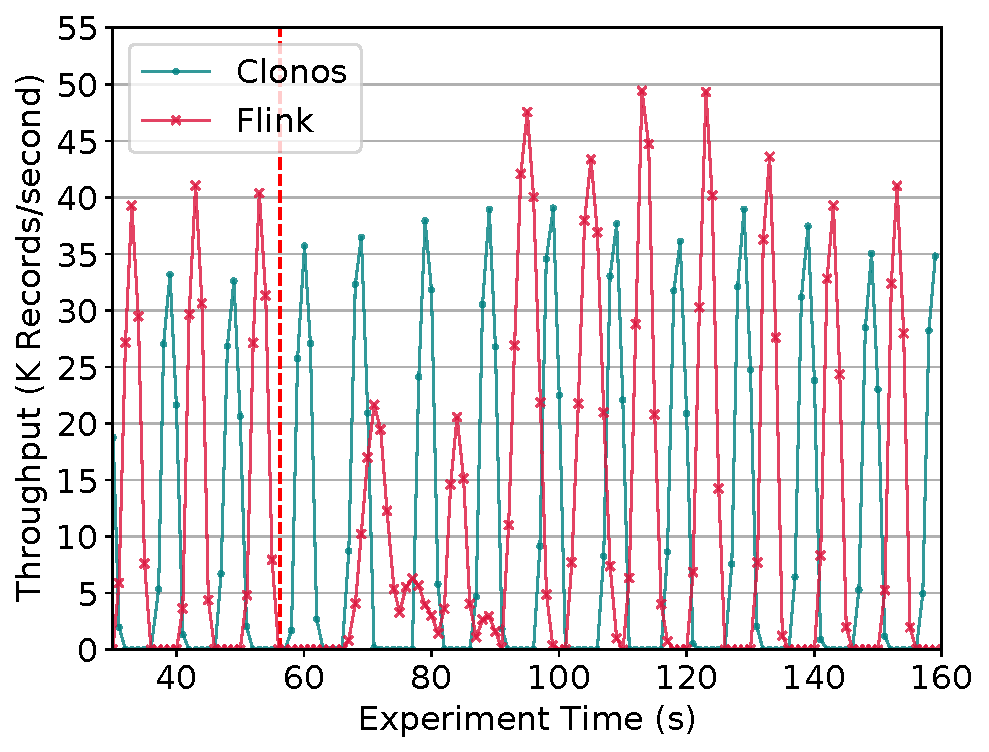
\includegraphics[width=\textwidth]{Figures/q8_failure_throughput.pdf}
		\caption{Q8: throughput}
		\label{fig:nexmark-q8-t}
	\end{subfigure}%
	~
	\begin{subfigure}[t]{.25\textwidth}
		\centering
		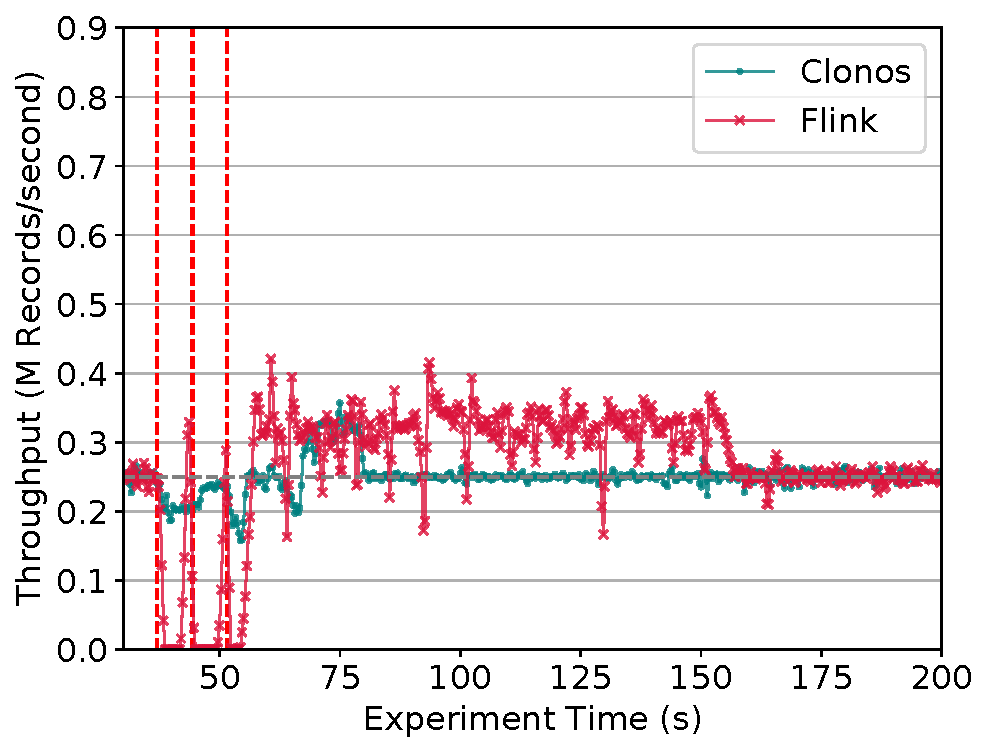
\includegraphics[width=\textwidth]{Figures/multiple_failure_throughput.pdf}
		\caption{Multiple: throughput}
		\label{fig:multiple-t}
	\end{subfigure}%
	~
	\begin{subfigure}[t]{.25\textwidth}
		\centering
		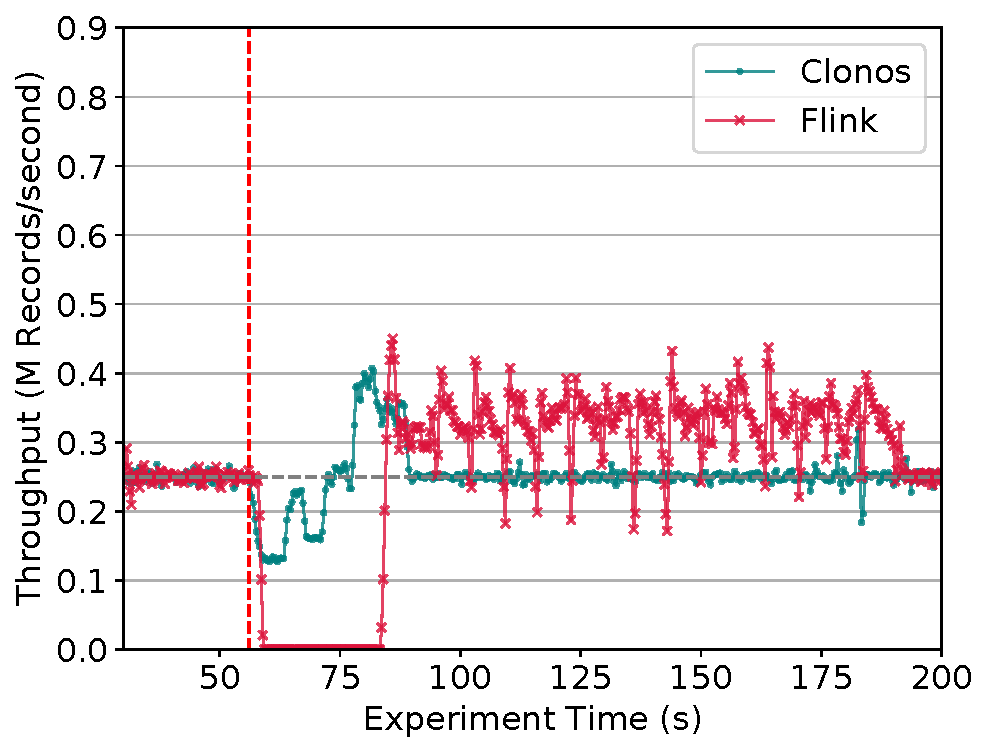
\includegraphics[width=\textwidth]{Figures/concurrent_failure_throughput.pdf}
		\caption{Concurrent: throughput}
		\label{fig:concurrent-t}
	\end{subfigure}%
	\vspace{-2mm}
	\caption{Failure experiments with realistic workload (left) and multiple/concurrent failures (right)}
  \label{fig:experiment-grid}
  	\vspace{-2mm}
\end{figure*}

For failure experiments we chose to present detailed throughput and latency metrics for two of the most interesting Nexmark queries: Q3, and Q8. In addition, we evaluate Clonos against Flink on multiple and concurrent failure scenarios using a synthetic workload. 
% \vspace{-3mm}

\para{Recovery Time} We define \textit{recovery time} to be the time between the instant that a failure takes place and the instant that the recovering system's observed latency has returned to values within 10\% of the pre-failure latency. This metric is used to evaluate a mechanism's ability to recover fast from a failure. Note that this metric also includes the time that a system needs to catch up with the input stream. Although Clonos is operational in less than a second, a lot of practical use-cases (e.g., credit card fraud detection) require that the system, after recovery, can also catch up with the input stream throughput and get back on track in order to process data as soon as it becomes available.


\vspace{3mm}
\begin{myframe}
\textbf{What is the performance of Clonos with respect to latency and throughput in the presence of single-operator failures?}
\end{myframe}
\vspace{2mm}

\para{Nexmark}
We focus on Q3 and Q8. 
Q3 performs a full history join and filtering operations,  while Q8 performs a windowed join, which explains the throughput spikes as we measure throughput at the job output sinks.
We have also experimented with Q4, Q5, and Q7 since they are the most complex queries, but those produce very few output records and they were inappropriate to plot and exemplify proper recovery times. In order to observe end-to-end latency, a regular amount of output records must be generated.

Figure~\ref{fig:nexmark-q3-l} shows that Clonos recovers within 10s by leveraging standby operators and local recovery.
After a sub-second switch to the standby operator, replaying the lost epoch took roughly 10s at which point a small number of queued records were emitted with 10s latency, before the system could catch up.
During this time, the alive tasks continue operating under regular latency.
Flink, however, loses availability on all tasks and takes at least 87s to recover and catch up. In addition, different output partitions recover at different speeds. This is indicated by the different lines of points visible in the plot.
In Figure~\ref{fig:nexmark-q8-l} we inject a failure to the join operator. Clonos recovers within 3s. Note that since we measure latency on the output records (end-to-end latency) the visible points arranged vertically signify records of different arrival times in their respective windows. The window range also explains the empty spots in the figure as the window fires every 10s.
Flink, on the other hand, takes more than 72s to fully recover.


In terms of \textit{throughput}, Figure~\ref{fig:nexmark-q3-t} depicts Clonos' ability to instantly recover the job's original throughput, while Flink experiences a downtime of multiple seconds and a turbulent recovery.
Notice how Clonos' throughput is barely affected following the failure. We can observe similar behavior in Figure~\ref{fig:nexmark-q8-t}.


\begin{comment}
In this series of experiments we aim at observing the performance of Clonos under different scenarios of failures. \autoref{fig:experiment-grid} depicts all the experiments that we chose to show. The top row shows latency and the bottom row shows throughput. The moments where we cause a failure are marked by a red vertical line. 

A job consists of Kafka source and sink operators with a number of map operators in between. 
The source and sink pull data from an input topic and push to an output topic, respectively. 
If a keyed stream is used, map operators manually shuffle their keys equally across all outputs. Otherwise, they simply forward their output to the next operator.

Six event generator nodes produce data into the input Kafka topic at a requested rate. 
Generators produce unique records including a timestamp of their generation time. This timestamp is later used to compute latency, by subtracting it from the time at which it is appended to the output topic.
\end{comment}

\vspace{3mm}
\begin{myframe}
\textbf{What is the performance of Clonos with respect to latency and  throughput in the presence of multiple failures?}
\end{myframe}
\vspace{2mm}

We perform our multiple and concurrent failure experiments at parallelism 5, operator graph depth 5, checkpoint interval 5 seconds, and per-operator state size of 100 MB. Specifically, Figures \ref{fig:multiple-l} and \ref{fig:multiple-t} depict an experiment where there are three failures with a 5-second interval, while Figures \ref{fig:concurrent-l} and \ref{fig:concurrent-t} depict an experiment with three concurrent failures. 
The failures are sequenced, meaning the failed operators have connected dataflows. 
We observe that independently of the frequency of failures (whether they are staggered or concurrent), Clonos' recovery behaves similarly. Before the downstream failures can be recovered, the upstream failures must finish recovering, such that they can replay their in-flight logs.
Only partial throughput is lost during recovery, as records continue to flow through causally unnaffected paths even though shuffle connections are used. Similarly, latency is only increased on a small subset of records flowing along causally affected paths and latency quickly returns to its pre-failure value.

\vspace{-5mm}
\subsection{Memory Usage}
The memory usage of Clonos is completely bound by the size of the buffer pools configured (\autoref{sec:in-flight-design}).
We have experimented with different memory sizes and spill strategies for the storage of the in-flight record log as well as determinants. 
We have observed that while the spill-buffer strategy is much more conservative memory-wise, it leads to poorer and less predictable performance. The spill-threshold strategy presents deteriorating performance under 50MBs of space and has diminishing returns above 80MBs.
%We have observed that throughput would only deteriorate if the in-flight log was given less than 50MBs of space, while any value over 80MBs did not yield any improvements in throughput.
Thus, all experiments used 80MBs of in-flight log space per task.
When the in-flight record log would become larger than the available memory, the log spills buffers to disk.
Since both reading and writing to it have a sequential access pattern, the "spill-threshold" strategy (\autoref{sec:in-flight-design}) yielded the best results.
The size of the determinant buffer pool has no effect on performance, but too small of a buffer pool may lead to deadlocks. 
Experimentally, we have found that for DSD=1 a determinant buffer pool of size 5MB is more than sufficient for most workloads. When DSD=Full, this value must be increased as D grows, as more logs are replicated.





\section{Related work}
\label{sec:related-work}

Our contributions are related to fault tolerance, high availability, and causal logging.
An elaborate study of fault tolerance and high-availability in stream processing is provided in a survey~\cite{fragkoulis2020survey}.

\subsection{Fault Tolerance}
A number of early stream processing systems provided fault tolerance, such as Aurora~\cite{CherniackBB03} and Borealis~\cite{BalazinskaBM05}. However, most fault tolerance approaches of the time did not recover a system-wide consistent state  with very few exceptions~\cite{Shah2004highly}.
More recent systems like Apache Flink~\cite{CarboneKE15}, IBM Streams~\cite{SilvaZD16}, and Microsoft Trill~\cite{ChandramouliGB15}, achieve consistent exactly-once fault tolerance with global rollback recovery as described in \autoref{sec:background}. Other systems, such as Storm~\cite{ToshniwalT14}, Heron~\cite{KulkarniBF15}, and Samza~\cite{NoghabiPP17}, implement at-least-once consistency guarantee.
Streaming systems to date increasingly try to handle failures locally, that is, without disrupting a job or regions of it, but only its failed components.
Apache Spark~\cite{ArmbrustDT18} performs exactly-once local recovery but in a micro-batch processing model and assuming an idempotent sink that ignores already produced results on recovery.
% by a) checking in a write ahead log which is the last committed micro-batch, b) loading that batch's state in its state store, and c) replaying the micro-batches following the last committed batch in order to reconstruct the system's state.

Consistent local recovery is offered by SEEP~\cite{FernandezMK13} and its extension based on stateful dataflow graphs (SDG)~\cite{FernandezMK14}, Timestream~\cite{QianHS13}, Streamscope~\cite{LinHZ16}, and Rhino~\cite{delmonte2020rhino}. However, none of these systems supports nondeterministic computations and they make strong assumptions about input order.
The only stream processing system that delivers consistent local recovery and can support nondeterministic computations with minimal assumptions is Millwheel~\cite{akidau2013millwheel}. However, Millwheel performs a transaction per record per operator on Spanner~\cite{spanner}. Spanner, to achieve low latency, depends on atomic clocks to operate which do not exist in commodity clusters. Clonos can provide Millwheel's guarantees and consistency on commodity hardware.
Table~\ref{tab:determinism-assumptions} summarizes all systems' determinism assumptions.




\subsection{High Availability}

Existing work on high availability in stream processing~\cite{Hwang2005HAA} proposes active replication~\cite{BalazinskaBM05, Shah2004highly}, passive replication~\cite{HwangX07, KwonB08}, hybrid active-passive replication~\cite{HeinzeZ15, SuZ16}, or models multiple approaches and evaluates them with simulated experiments~\cite{ChandramouliG17, Hwang2005HAA}. These approaches either constrain operator logic or support weaker than exactly-once consistency guarantees.
Clonos delivers high availability based on passive replication by substituting only the failed tasks. At the same time Clonos maintains exactly-once consistency guarantees that cover nondeterministic computations using causal logging on a feature-rich production-grade system.


\begin{table}[t]
  \caption{Assumptions of related work}
  \label{tab:determinism-assumptions}
  \vspace{-2.5mm}
  \small
  \begin{tabular}{p{0.11\textwidth}|p{0.32\textwidth}}
      \toprule
      \textbf{System} & \textbf{Assumptions} \\
      \bottomrule\toprule
      Millwheel \cite{akidau2013millwheel} & Scalable, transactional backend (Spanner) \\ \hline
      Streamscope \cite{LinHZ16} & Deterministic computations and input \\\hline
      Timestream \cite{QianHS13} & Deterministic computations and input \\\hline
      SEEP \& SDG \cite{FernandezMK14}, Rhino \cite{delmonte2020rhino} & Deterministic computations, monotonically increasing logical clock, records ordered by time.\\\bottomrule
      \toprule
  \end{tabular}
\end{table}

\subsection{Causal Logging}

We presented causal logging~\cite{elnozahy1994manetho, elnozahy2002survey}  in \autoref{sec:background}. 
We have elaborated both the system design and implementation aspects of the causal log in Section~\ref{sec:design} and the nondeterministic aspects in Section~\ref{sec:nondeterminism}.

Among streaming systems, Timestream~\cite{QianHS13} and Streamscope~\cite{LinHZ16} use an optimistic logging-inspired dependency tracking approach, which records input and output dependencies in computations and uses them to rebuild the state if needed.
Instead, Clonos records all nondeterministic events and the order of execution. By additionally respecting the always-no-orphans condition, Clonos can guarantee consistent localized recovery.

Closest to the spirit of Clonos is lineage stash~\cite{wang2019lineage}, which uses causal logging to provide exactly-once consistency with local recovery for nondeterministic operators. However, it does not support important nondeterministic functions in stream processing, such as timer-based services much needed for processing time windows and watermarks required for progress tracking and out-of-order data.
In addition, it uses a micro-batch architecture while Clonos implements continuous data processing. Finally, Clonos also addresses issues of high availability with standby tasks, state shipping and reconfiguration.


\section{Conclusions}
\label{sec:conclusions}

In this paper we presented Clonos, a fault-tolerance and high-availability method built in Apache Flink as a replacement for its current fault tolerance mechanisms. Clonos, to the best of our knowledge, is the first fault tolerance mechanism which is applicable to a real, production-grade system and achieves consistent local recovery, high availability, and the flexibility of nondeterministic computations. Clonos has been a substantial engineering effort within our team (more than 20K LOC), which still continues improving the overhead of causal logging. Our experiments so far have shown that Clonos can be competitive (5-24\% overhead in throughput and latency) with the current fault-tolerance mechanism of Flink which is industry-proven and serves billions of events every day, in multiple industries. 
At the moment, we are extending our work into reducing the overhead of causal logging through compressed data structures and extending Clonos' guarantees to low-latency exactly-once output.


\para{Acknowledgements} This work has been partially funded by the H2020 project OpertusMundi No. 870228, and the ICAI ``AI for Fintech Lab" project. Experiments were carried out on the Dutch national e-infrastructure with the support of SURF Cooperative.



\balance

  \bibliographystyle{ACM-Reference-Format}
  \bibliography{hastreaming}
  

\balance
  
  \end{document}
  \endinput
  %%
  %% End of file `sample-sigconf.tex'.
  
